\chapter{Virtual Spaces}
\label{ch:virtual}

Over the past twenty years, the prospect of visiting a virtual world different from our own world has moved from being strictly the domain of imagination to being widely accessible. What started as worlds presented through text-based descriptions and interacted with through typed commands have evolved into rich graphical and sensorial experiences that became rapidly accessible to mass audiences. The argument for virtual worlds has always had a revolutionary tone. Virtual worlds might, for example, suppress the prejudices of offline society by hiding identity information, breaking down the boundaries of distance, and making experiences broadly accessible that might not otherwise be feasible. Perhaps we could even build a new virtual society, one that is better than our own. These utopian visions are attractive precisely because the urge to grow beyond the confines of everyday experience is so strong.

This vision was so attractive that in the mid 2000's the market research firm Gartner famously predicted in 2007 that by the end of 2011, ``80 percent of active Internet users (and Fortune 500 enterprises) will have a `second life', but not necessarily in \emph{Second Life}.'' \citep{Anonymous:2007wz}. This has not come to pass. Linden Lab has stopped publishing public usage data, but it is clear by comparing its cultural impact to systems like \emph{Facebook}, \emph{Twitter}, and \emph{YouTube} that \emph{Second Life} has been almost completely eclipsed in the public imagination by other types of mediated social experiences. Despite this shift, it is still productive to consider to this period where virtual worlds were viewed as strong potential venues for mediated social interaction. What attracted us to these experiences in the first place? Why did these experiences ultimately fail to catch people's imaginations? Are there aspects of ``virtual'' experiences that were left behind in the shift away from a ``virtual'' approach that might be valuable components of more modern experiences? Why did the reality of accessible virtual worlds fail to live up to their revolutionary, utopian promise?

In this chapter I will address these questions through an analysis of the properties of virtuality and a pair of design projects: \emph{Information Spaces} and \emph{Presentation Spaces}. Although these projects do not exemplify the best sorts of \emph{in situ} research, they serve as conceptual arguments about how we might think about designing virtual experiences that take advantage of what virtuality offers designers that is missing in other approaches to mediated interaction. The approaches I will describe contrast with the much of the interface design work in virtual worlds in this period that focused on replicating the forms of offline experiences and expecting them to have the same properties when transplanted into a virtual context.

Although in its specifics this argument is perhaps a little dated and unlikely to apply directly in the future (barring a resurgence of virtual world design), it can be seen also as an argument for how to do a close reading of the properties of a platform and letting those properties guide a design that is closely adapted to its tools. Considering virtual worlds in this detail helps highlight some of the taken-for-granted assumptions about non-virtual design.

In a larger sense, a deep discussion of virtuality will also demonstrate how the core research themes of this thesis--grounding, non-verbal actions, and attention--operate in an unfamiliar context. Although readers might be unfamiliar with operating in a virtual world environment, this unfamiliarity will help address these research themes without preconceptions.

I open this chapter with some background on my structural approach to thinking about virtual worlds. I will describe how spatiality, dimensionality, representation, and presence interact with the social experiences that a world can effectively support. I will argue that spatiality and presence are the core differentiating factors that define a virtual world, and the two projects that I describe in this chapter try to make maximum use of those factors. Finally, I close the chapter with a reflection on why virtual worlds have failed to gain wide-spread traction and on whether the work in this chapter might be effective if re-imagined outside a virtual world platform. 

% I open this chapter with a discussion of what precisely defines a ``virtual world'', focusing on the distinction between spatiality and dimensionality. 
% 
% 
% % TODO this isn't actually how I open, fix this.
% 
% 
% 
% 
% I will defer an analysis of why this might have happened for later in this chapter, but 
% 
% 
% As with many technology trends, there is a sort of pendulum that swings between different design strategies. Our earliest mediated social experiences (like email and chat) were primarily text-based media. 
% 
% 
% 
% This chapter explores some of my early work in the virtual world space and draw comparisons between 


\section{Characterizing Virtual Worlds}

Though is no widely agreed upon typology of virtual worlds (though there are many examples, e.g. \citep{Koster:2007wg} or \citep{Bartle:2003up}), there are a few general categories that scholars of virtual worlds tend to agree are important to properly describe the kind of worlds that this thesis is concerned with.\sidenote{This section draws heavily from \citep{Harry:2008vx}.}

The two major axes on which virtual worlds can be organized (as proposed by \citet{Bartle:2003up} are agency (which Bartle calls `change') and persistence. Agency is a broad term that is the set of things that someone can do in a world. Agency can be thought of as the interface that you have onto the world. For example, the agency of players in a chess game is limited. When it's their turn they can move their own pieces in certain prescribed ways. Moving pieces is the agency players have in the chess game. In virtual worlds, agency becomes a bit more elaborate and includes movement, avatar customization, communication, object creation, etc. Different worlds have different sets of actions that an avatar can do, and I describe them as having different kinds of agency.

Persistence is the ability of the world to remember events that change something about the world. For example, if you create an object in a persistent virtual world you can expect that the object will be there when you return. This is in contrast to worlds where changes aren't saved for very long. Multiplayer first person shooter games are a good example of this---you interact with a rich three-dimensional world and might change it by dropping weapons, causing explosions that change the appearance of part of it, or by destroying certain objects in the environment. None of those changes will remain in that world the next time you play, though. It will be wiped clean and you'll have a fresh copy of the original space. These spaces often even revert to their original state after a few minutes: bodies disappear, dropped weapons fade, and explosion marks are removed. 

Certainly, these axes are not perfectly distinct (worlds with limited agency often have low persistence as well), but they serve as good organizing principles. For the most part, modern virtual worlds have high levels of agency but relatively low levels of persistence. In \emph{World of Warcraft} for instance, players can kill monsters in the world, but the monsters will always reappear a few minutes later. There are virtually no actions players can take that modify any aspect of the world apart from killing computer controlled characters. Rich agency exists almost entirely in the relationships between players and the organizations they form. Worlds like this have proven to be commercial successes because they are more resistant to disruptive behavior aimed at degrading other players' experiences, but they also rule out many of the interesting opportunities that virtual spaces offer over physical spaces.

The best recent example of a world that offers that kind of rich agency and persistence is \emph{Second Life}, a world developed by Linden Lab. \emph{Second Life} is a free application that connects to a single monolithic ``Grid'' of \emph{Second Life} servers that provide a mostly continuous (flat) virtual space in which avatars can own land and items, build clothing, buildings, or vehicles, and embed behavioral scripts in their creations. The world also provides an economic system with its own currency system (the Linden Dollar, L\$), which is exchangeable at a fixed rate for US Dollars on a currency exchange that Linden Lab manages. The community that has arisen around \emph{Second Life} is extraordinarily diverse and rich, but an in depth discussion of its dynamics is beyond the scope of this chapter. There are a number of books that describe the history and culture of \emph{Second Life}, which provide a good introduction to that topic, however. \citep{Au:2008va, Ludlow:2007uu} For my purposes, \emph{Second Life} is critical as an example of a world in which avatars have a considerable amount of control over the design of environments, and so \emph{Second Life} has been instrumental in developing an intuition for how virtual spaces influence the behavior of people in them. It has also been useful as a platform for exploring the design space of algorithmic architecture. For much of this chapter, I will turn to \emph{Second Life} as a source of inspiration, as well as to draw comparisons between the general model for virtual architecture that I explore in this thesis and the model that \emph{Second Life} embodies.

The following sections lay out the pieces of what might make something feel like a world. There is not clear set of necessary and sufficient conditions for world-ness. Instead, these sections introduce a series of concepts that all lend-themselves to fostering a sense of world-ness. These concepts are Representation, Spatiality, and Presence. 

\subsection{Representation and Function}
Specific features of both physical spaces and virtual spaces can be thought of as serving symbolic and functional purposes. As virtual spaces were first being conceived it was not obvious that they would draw their symbolism heavily from physical spaces \citep{Novak:1991ue}. Novak would no doubt be surprised to see how familiar the design elements of can be. In \emph{Second Life}, for instance, there are countless recreations of both specific architectural landmarks as well as buildings that ape familiar architectural styles. Those buildings in turn are filled with rooms furnished in a way that would not stand out in the least from their real world analogs. Why is it that, free of the natural laws of the physical world, so much of virtual world design is concerned with recreating familiar physical spaces?

This focus on familiar representations serves a number of important social roles. First, it functions much like the identity signals do in physical fashions. Although choosing and furnishing a virtual house is substantially less costly than its physical analog, it is still a strong demonstration of taste that helps visitors to virtual spaces understand something about the person who assembled them, much like a personal homepage or profile page might on the Web. And though the price of virtual items may be substantially less than the physical artifact it mimics, virtual economies usually have some sense of relative value that allow these items to also function as signals of wealth.

\begin{figure*}[t]
	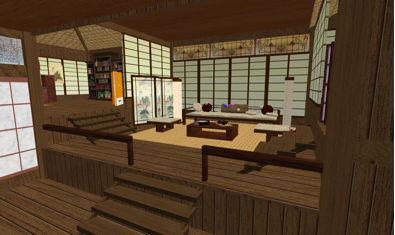
\includegraphics{figures/asian_home.png}
	\caption{A \emph{Second Life} home decorated in an Asian style.}
	\label{fig:asian_home}
\end{figure*}

The second important social role is in building spaces that contextualize behavior. Visitors to virtual worlds are forced to reform their notions of socially acceptable behavior in virtual spaces. It is substantially easier to make meaning from a virtual space built to look like something familiar than something abstract. In this way, avatars in virtual spaces can reasonably expect that spaces that look like virtual museums, dance clubs, meeting rooms or houses should be used for virtual analogs of what one might do in their offline equivalent. This argument is analogous to Norman's, with respect to the design of interactions with physical objects \citep{Norman:2002tv}. He describes how physical objects use metaphors to demonstrate affordances. Metaphors imply a conceptual model that makes it easier for people to make deductions about what how their interactions with the system will affect it. In a very similar way, literal representations in virtual architecture serve as behavioral affordances. They use architectural metaphors to imply what the social model of the space should be. 

Although literal representational techniques serve effectively as identity signals and behavioral affordances, this does not mean that they are the only way to do effective design work in virtual worlds. Indeed, the work in this chapter will try to demonstrate an alternate approach.

I will describe spaces which not just look different and imply that different behaviors are expected but spaces that actually have different functional affordances that make certain activities more or less effective in a particular space. Functional affordances are those that are not simply based on what the space looks like, but what aspects of the world that are algorithmic and reactive in some way. We should treat virtual space as a new medium that has its own strengths and weaknesses instead of trying to create the experience of ``being there.'' This distinction is best understood through analogy to how symbolism and function interplay in two kinds of physical spaces: cathedrals and nightclubs.

\begin{figure*}[t]
	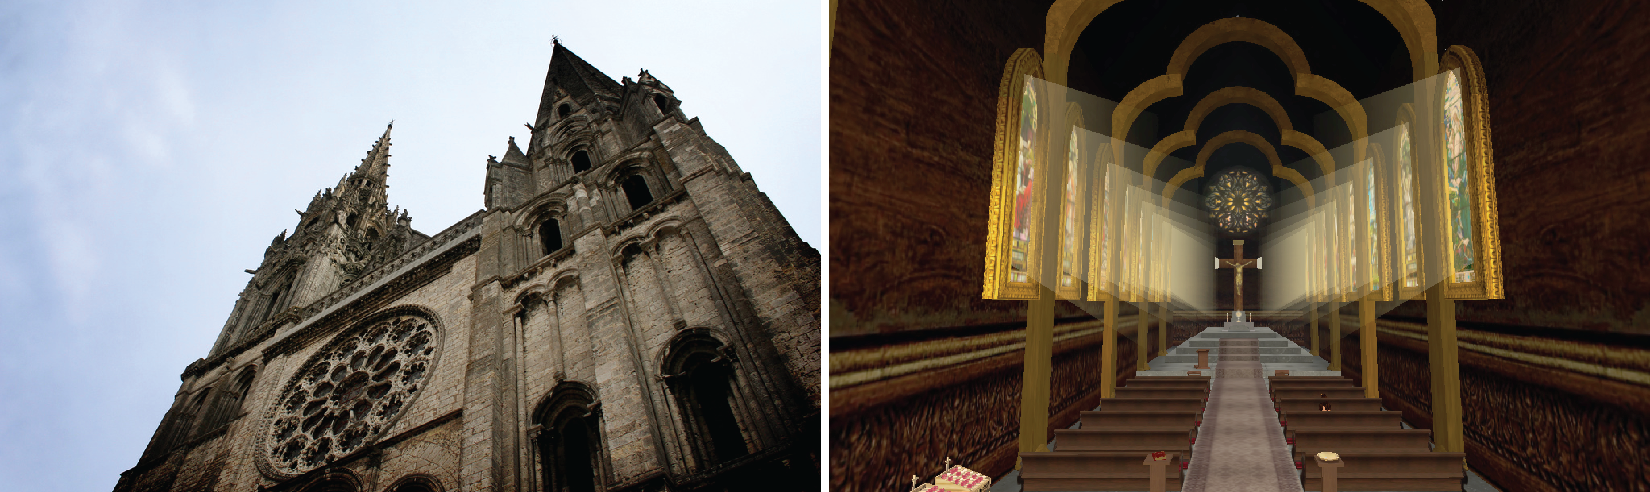
\includegraphics{figures/cathedral_comparison.png}
	\caption{Left: Photo of a cathedral, courtesy of flickr user glynnis. Right: Screenshot of a cathedral in \emph{Second Life}.}
	\label{fig:cathedral_comparison}
\end{figure*}

The form of a classical cathedral is rich with religious symbolism that informs the overall structure of the building, detailed adornments, lighting, and scale. It also has certain functional affordances. The space is designed such that a speaker at the podium can be easily seen and heard by the people in the pews. This also means that the whole congregation will easily hear any noises from the pews. This encourages parishioners to be quiet, and re-enforces the power dynamics inherent to the church; visitors are not there to interact with each other.

Nightclubs use acoustics and lighting to create a very different kind of space. Although the precise form of clubs varies, the functional aspects of clubs are often quite similar. Loud music makes it hard to hear people far away, which both forces people to be close together to talk and makes it hard to be overheard. In this environment, it is easy to have intimate conversations. Low lighting makes it difficult to see people, hear them, and identify them. This creates a situation in which people must fill in information about each other because the environment makes that information hard to get. Darkness and candlelight in a cathedral would have a different effect---the functional and cultural/symbolic meanings are interwoven.  The nightclub is known to be about hedonism and escape; the cathedral, for the believer, about spiritual, solemn, and perhaps frightening/awe-inspiring experience.

Lighting and acoustics are two aspects of what I call ``functional'' aspects of space. They operate mostly independently of how a space looks (that is to say two spaces could look the same but have different acoustics) and both respond to people's actions in the space as well as mold those actions. These two examples demonstrate how the functional side of spaces has a big impact on what kind of activities make sense in them. You would not, for instance, try to hold a business meeting in a nightclub or hold small group discussions in a cathedral. Yet virtual spaces very rarely have this kind of adaptability to their designed purposes. You could, in a world like \emph{Second Life}  hold a business meeting in a virtual night club with no particular ill effects. It would be a strange juxtaposition, but the location would be only a visual distraction, not a major impediment to having a conversation. The heart of this chapter is to show how building virtual spaces that exhibit some of these same sorts of properties might create compelling virtual experiences that are competitive with non-virtual interfaces.

\begin{figure*}[t]
	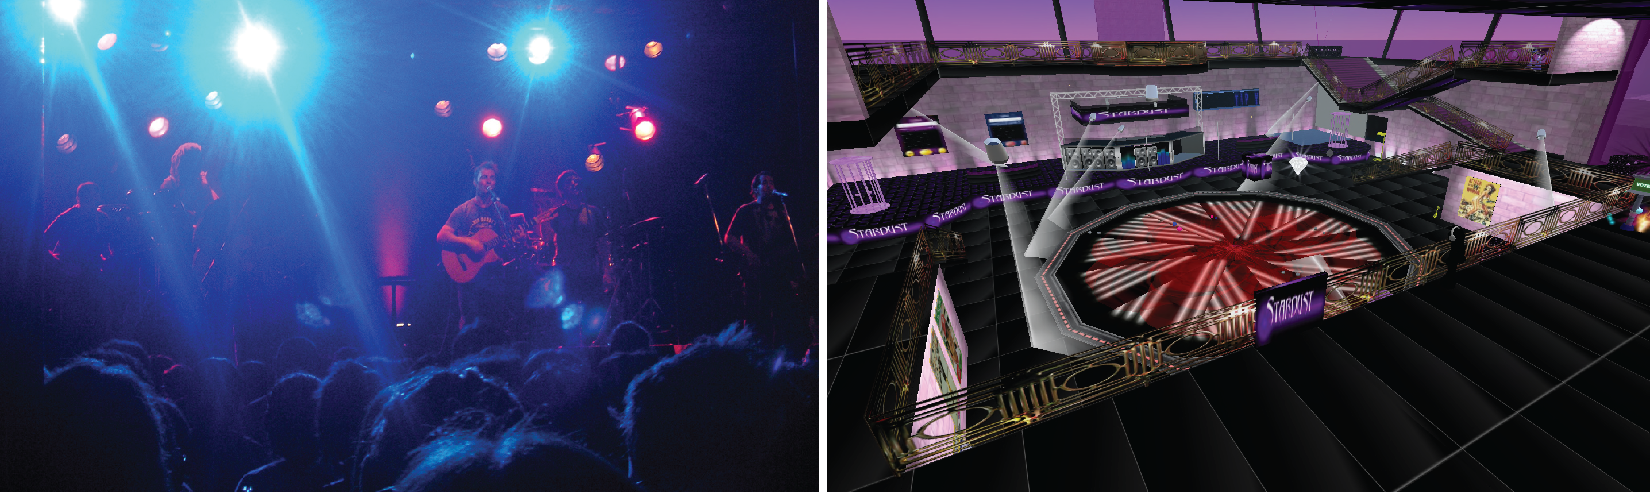
\includegraphics{figures/club_comparison.png}
	\caption{Left: Photo of a nightclub. Right: An empty nightclub in \emph{Second Life}.}
	\label{fig:nightclub_comparison}
\end{figure*}

\subsection{Dimensionality and Spatiality}
\begin{quotation}
One question we are frequently asked is why use 3D for a collaboration environment? While it might be possible to build a 2D tool with functionality similar to [Project Wonderland], the spatial layout of the 3D world coupled with the immersive audio provides strong cognitive cues that enhance collaboration. For example, the juxtaposition of avatars in the world coupled with the volume and location of the voices allows people to intuit who they can talk to at any given time. The 3D space provides a natural way to organize multiple, simultaneous conversations. Likewise, the arrangement of the objects within the space provides conversational context. If other avatars are gathering near the entrance to a virtual conference room, it is a good guess that they are about to attend a meeting in that space. It is then natural to talk to those people about the content or timing of the meeting, just as you would if attending a physical meeting. In terms of data sharing, looking at objects together is a natural activity. With the 3D spatial cues, each person can get an immediate sense of what the other collaborators can and cannot see. --- \emph{Sun Labs, describing the features of a virtual world that made it a compelling space for group work.}\citep{Anonymous:tv}
\end{quotation}

It's difficult to pin down exactly what makes a virtual world a world. In the previous section we draw the distinctions of agency and persistence from the literature. These are useful for distinguishing between different sorts of world, but are not sufficient to distinguish worlds from non-worlds. Another attractive potential to draw a distinction between worlds and non-worlds might be a certain immersive representation. When we think about immersion, we typically presume that means a three dimensional representation. 

The role of dimensionality in virtual worlds is subtle. Over the course of my work, I have shifted from focusing on three dimensional representations to two dimensional representations. Although this shift leads to a radical change in how people view a space (few people look at a two dimensional web application and say ``this is a virtual world!''), it is perhaps not as fundamental a shift in metaphor as you might initially suspect. This section draws a distinction between the dimensionality of a system (which is primarily a representational quality) and the spatial properties of a system (which is primarily an active, functional quality). Although often conflated, these are separate qualities. Both can promote a sense of world-ness, but it is quite possible to have a feeling of occupying a world without a three dimensional representation, provided there is some sort of spatial structure.

The dimensionality of a world is an aspect both of its display and its abstract data representation. Objects in a three-dimensional world have a position in three-dimensional space, a solid volume, and an orientation in three rotational axes. In an intuitive sense, a three-dimensional virtual world looks a lot like the three-dimensional physical world we are used to. The programmatic representation of the world need not be bound to its visual representation, however. It is possible to build a three-dimensional representation of a fundamentally two-dimensional world. The MASSIVE system demonstrates this nicely; they had both a three-dimensional visual client and a text based two-dimensional client. Both clients could almost completely represent the world state. As a world, MASSIVE had no vertical dimension, so its three-dimensional representation was simply a skin on a two dimensional world. \citep{Greenhalgh:1995gz} What's important, though, is drawing a distinction between the dimensionality of the world itself and the dimensionality of its visual representation---they need not necessarily be the same thing.

The perspective on a world is an important related aspect of the world that is related to its dimensionality. Three-dimensional worlds have two major perspective options: first person and third person. In a first person perspective, the user views the world as if the camera was placed where the eyes of the avatar would be. If they see their own body at all, it is usually only their hands or feet. In this mode, the user literally inhabits the body of avatar and becomes that character in a significant way. In a third person perspective, the user sees their character from a camera that is usually behind them looking down. This provides a better sense of the world around their character, but can sacrifice some immersion by showing the avatar animating itself or looking different than a user's own vision of them. The choice of perspective is primarily one of immersion: first person views are more immersive than third person views. In two-dimensional worlds, third person views are essentially the only option. A first-person two-dimensional view would be Flatland \citep{Abbot:1899th}, with all of the challenges of navigation and interaction explored in that book.

Spatiality is harder to precisely describe because almost without exception virtual worlds are all spatial in some way or another. MUDs offer perhaps the best starting point as one of the least spatial examples of a virtual world. In a MUD, players occupy discrete rooms. Each room can contain many players and objects, and is connected to other rooms through a series of nominally spatial relationships. For instance, from a given room, you might direct your character to move north which would move your character into the room that the system thinks is north of the room you were in. Although this model is spatial in the sense that you can be closer or farther from people, avatars in early MUDs had little agency or perception of events anywhere but their current room. In a given room, there is no functional spatiality; all players and objects occupy a sort of indistinct space where they could hear and interact with each other, but have no finer position than the room itself. As a result, there was no context for using the kinds of spatial language that make spatiality so useful. A player couldn't describe an object as being ``the thing on your right.''

Furthermore, the connections between rooms themselves were not reliably spatial in any particular way. Although they were ostensibly arranged in cardinal directions, there is no enforcement of ``normal'' spatiality. A series of rooms could easily fold back on itself such that moving north a few times would return you to the room you started in. Different routes out of a single room might all go to the same room. Paths might even behave differently in different directions; moving north from one room to another, and then south to try to get back again might not necessarily take you back to where you started. In this way, even an ostensibly spatial metaphor breaks down and fails to convey the contextual and perceptual benefits of true spatiality. In contrast, a world where objects and avatars have distinct discrete locations immediately confers these benefits. Avatars can indicate group membership by avatar proximity, can have a shared visual reference point, and so can communicate about objects behind or to the right of other avatars. 

Returning to the quote about \emph{Project Wonderland} that introduced this section, I argue that they are conflating notions of dimensionality with spatiality. All of the beneficial features that are ascribed to a ``3D world'' are more properly ascribed to a world with rich spatiality. A two-dimensional virtual conference room can have an entrance where avatars congregate just as easily as a three-dimensional world. Two-dimensional worlds confer the same benefits regarding shared gaze, too. An avatar in a two dimensional world can infer another avatar's view on that world in the same way they might in a three-dimensional world. These are all properties of a world's spatiality and not its dimensionality. Although the work I describe in this chapter is two dimensional, I have maintained spatiality wherever possible. This maintains many of the benefits in the introductory quote while avoiding the many challenges of working in three dimensions. Translating this design approach into three dimensions is certainly possible, although maintaining spatiality in three dimensions requires a certain vigilance. \emph{Second Life} is an instructive example here. Avatars in \emph{Second Life} freely move their cameras with no external representation of its current location. As a result, an avatar's position in the space has little to do with their current view, and so spatial language isn't necessarily that useful.  Chapter 4 demonstrates how three-dimensional spaces can be used with this same approach, and similar analogs could be built for essentially all the zones and ideas presented here.

While I believe that worlds that are fundamentally two-dimensional are not inherently less spatial than their three-dimensional counterparts, there is something to be said for the representational language (as opposed to the functional or algorithmic language) of three-dimensional spaces. As discussed in the previous section, three-dimensional spaces tend to offer more legible spaces because they use a representational language that is familiar. Meeting rooms represented in three dimensions (or even some sort of isometric view) may be more obviously meeting rooms than the very abstract vector-graphics style rooms I show in this chapter. For my purposes, though, the dimensionality is not particularly important for demonstrating the design space. Instead, it is spatiality that is critically important for creating a sense of being in a world.

% TODO talk about the tradeoffs inherent to spatiality, per discussions with sinchan?

% TODO show pictures of both interfaces that promote a sense of presence (eg turntable) but aren't actually spatial? I had some thought about habbo hotel and that israeli chat system that I can't seem to recall just now. 

\subsection{Representation and Presence}

% add an argument here that the final component to world-ness is a representation of specific people. I'm not sure that's in the original thesis so it probably needs to be written from scratch.

The most visible distinction between world-like experiences and non-world like experiences is the way that people are represented. In a system like \emph{Second Life}, people are represented as quasi-realistic avatars. Not only do they look like people, they move and interact like people: they shift stance, walk, run, wave, and dance in more or less realistic ways. When these representations are combined with literally-designed spaces (that is, spaces that look like non-virtual spaces) it all starts to feel quite familiar and world-like.

This is clearly an attractive approach; it seems natural to expect that a software world that looks like the real world that is populated by people who move look and move like real people that it will be valuable. We'll defer a deeper discussion of why this is a bad assumption. Instead, I seek to place avatars on a continuum of representation strategies, any of which can support a sense of a sense of presence. This argument is analogous to the dimensionality and spatiality argument made in the previous section; spatiality is where the world-ness comes from, and you can create spatial experiences with a variety of dimensional choices. The same is true for representing people. What's important is that you foster a sense of presence, not that a particular representation is inherently superior.


There are a wide variety of representational strategies that focus on different aspects of someone's identity. Pseudonyms are widely used for their simplicity, but are nevertheless quite expressive. A name alone can paint an evocative picture of a person, although it might not mirror their offline identity presentation. \citep{Jacobson:1996tb} More elaborate representations can accumulate behavior in some social context like number of posts, number of friends, age in a community, or metrics representing the quality of one's contributions to the community. Image-based avatars like those on \emph{Facebook} and \emph{Twitter} add a more flexible visual vocabulary for representation that easily supports both photos that leverage offline representational strategies as well as more abstract and conceptual representations. Finally, pure self-description is quite common as well. Whether the third-person description style of MUDs, a one line ``bio'' on \emph{Twitter}, or the full suite of different tools that make up a profile page on \emph{Facebook}, online representations frequently employ text in a variety of ways. The properties of each of these strategies vary, but they all provide non-literal ways of creating a sense of identity online. 

Presence, however, is a different matter and is decoupled from representational strategy. We would probably not describe \emph{Facebook} as a virtual world not because its representations of people are a combination of text and photos, but because there is little sense of being in a space with someone. We are aware only of someone's actions, not their presence. Most asynchronous-oriented online experiences share this character. The space is well represented and we see the traces of someone's actions after they happen, but we don't see the presence of non-acting people in the space. Simply indicating in some way that other people are viewing the same document (as in \emph{Google Docs}) can be enough to create a sense of presence, even in the absence of a world more complicated than a simple text document. 


% Erm, this is an interesting argument but I'm afraid of making it too strongly without any actual research here. This was sort of okay in masters thesis land but is probably bad here. Return to this later and decide if I want/need it to be there.

% basically the plan is:
%  - talk about different strategies other than avatars
%		- performance based strategies on stackoverflow, forums
%		- image avatars (ala facebook, twitter)
%		- pseudonyms (everything)
%		- mention MUD self-descriptions 
%
% introduce the difference between facebook where you see the results of actions, but not the people doing the actions themselves. use room metaphor.
% this is the heart of the difference between representation and presence. few would describe facebook as a virtual world because there is little sense of the presence of others; someone who is not actively writing something on facebook has no representation. There is thus little sense that someone is actually present. We see the footprints but not the people. 
%
% IM distinction
% talk about text-based



\section{Information Spaces}
As a first step in exploring the potential of virtual architecture, I developed a space in Second Life that focuses on the social meaning that an avatar's position in a space can have and how that meaning can be augmented using some of the aggregative properties of virtual space. \citep{Harry:2008ww} This particular design is focused on meeting situations. In meetings with more than a few people, it can be challenging to understand other people's feelings about an issue, reach consensus, and influence others. In \citet{McGrath:1984un}'s terms, I'm focused on decision-making tasks, with an added interest in supporting some sorts of planning tasks like staying on an agenda and distributing tasks. The design addresses these collaboration challenges by creating a meeting space focused on non-verbal signaling using avatar positions. The main stage in this space is a chat or audio conversation, while the side stage is the positions of avatars and associated visualizations. The goal of this side stage is to help manage the decision-making process by creating visualizations that make magnify and make persistent avatar movement within the meeting space in a way that encourages participants to use their avatar's position in a more performative fashion. To support this use, I built a range of social utilities---systems that make visible properties of avatars' social behavior in the space. These visualizations are all controlled by a centralized dashboard, such that the nature of the space can be controlled by the moderator, much like a meeting organizer might set up the chairs and projector in a physical meeting room depending on the kind of meeting they were having. An overview of the meeting space can be found in  Figure \ref{fig:information_space_overview}.\sidenote{This section draws heavily from \citep{Harry:2008vx}.}

Beyond the space itself, I also developed a number of meeting support widgets that can augment a virtual meeting room. These widgets are not strictly architectural, but they show how different kinds of tools could create virtual spaces that are more or less appropriate for a certain kind of meeting.

\begin{figure*}[t]
	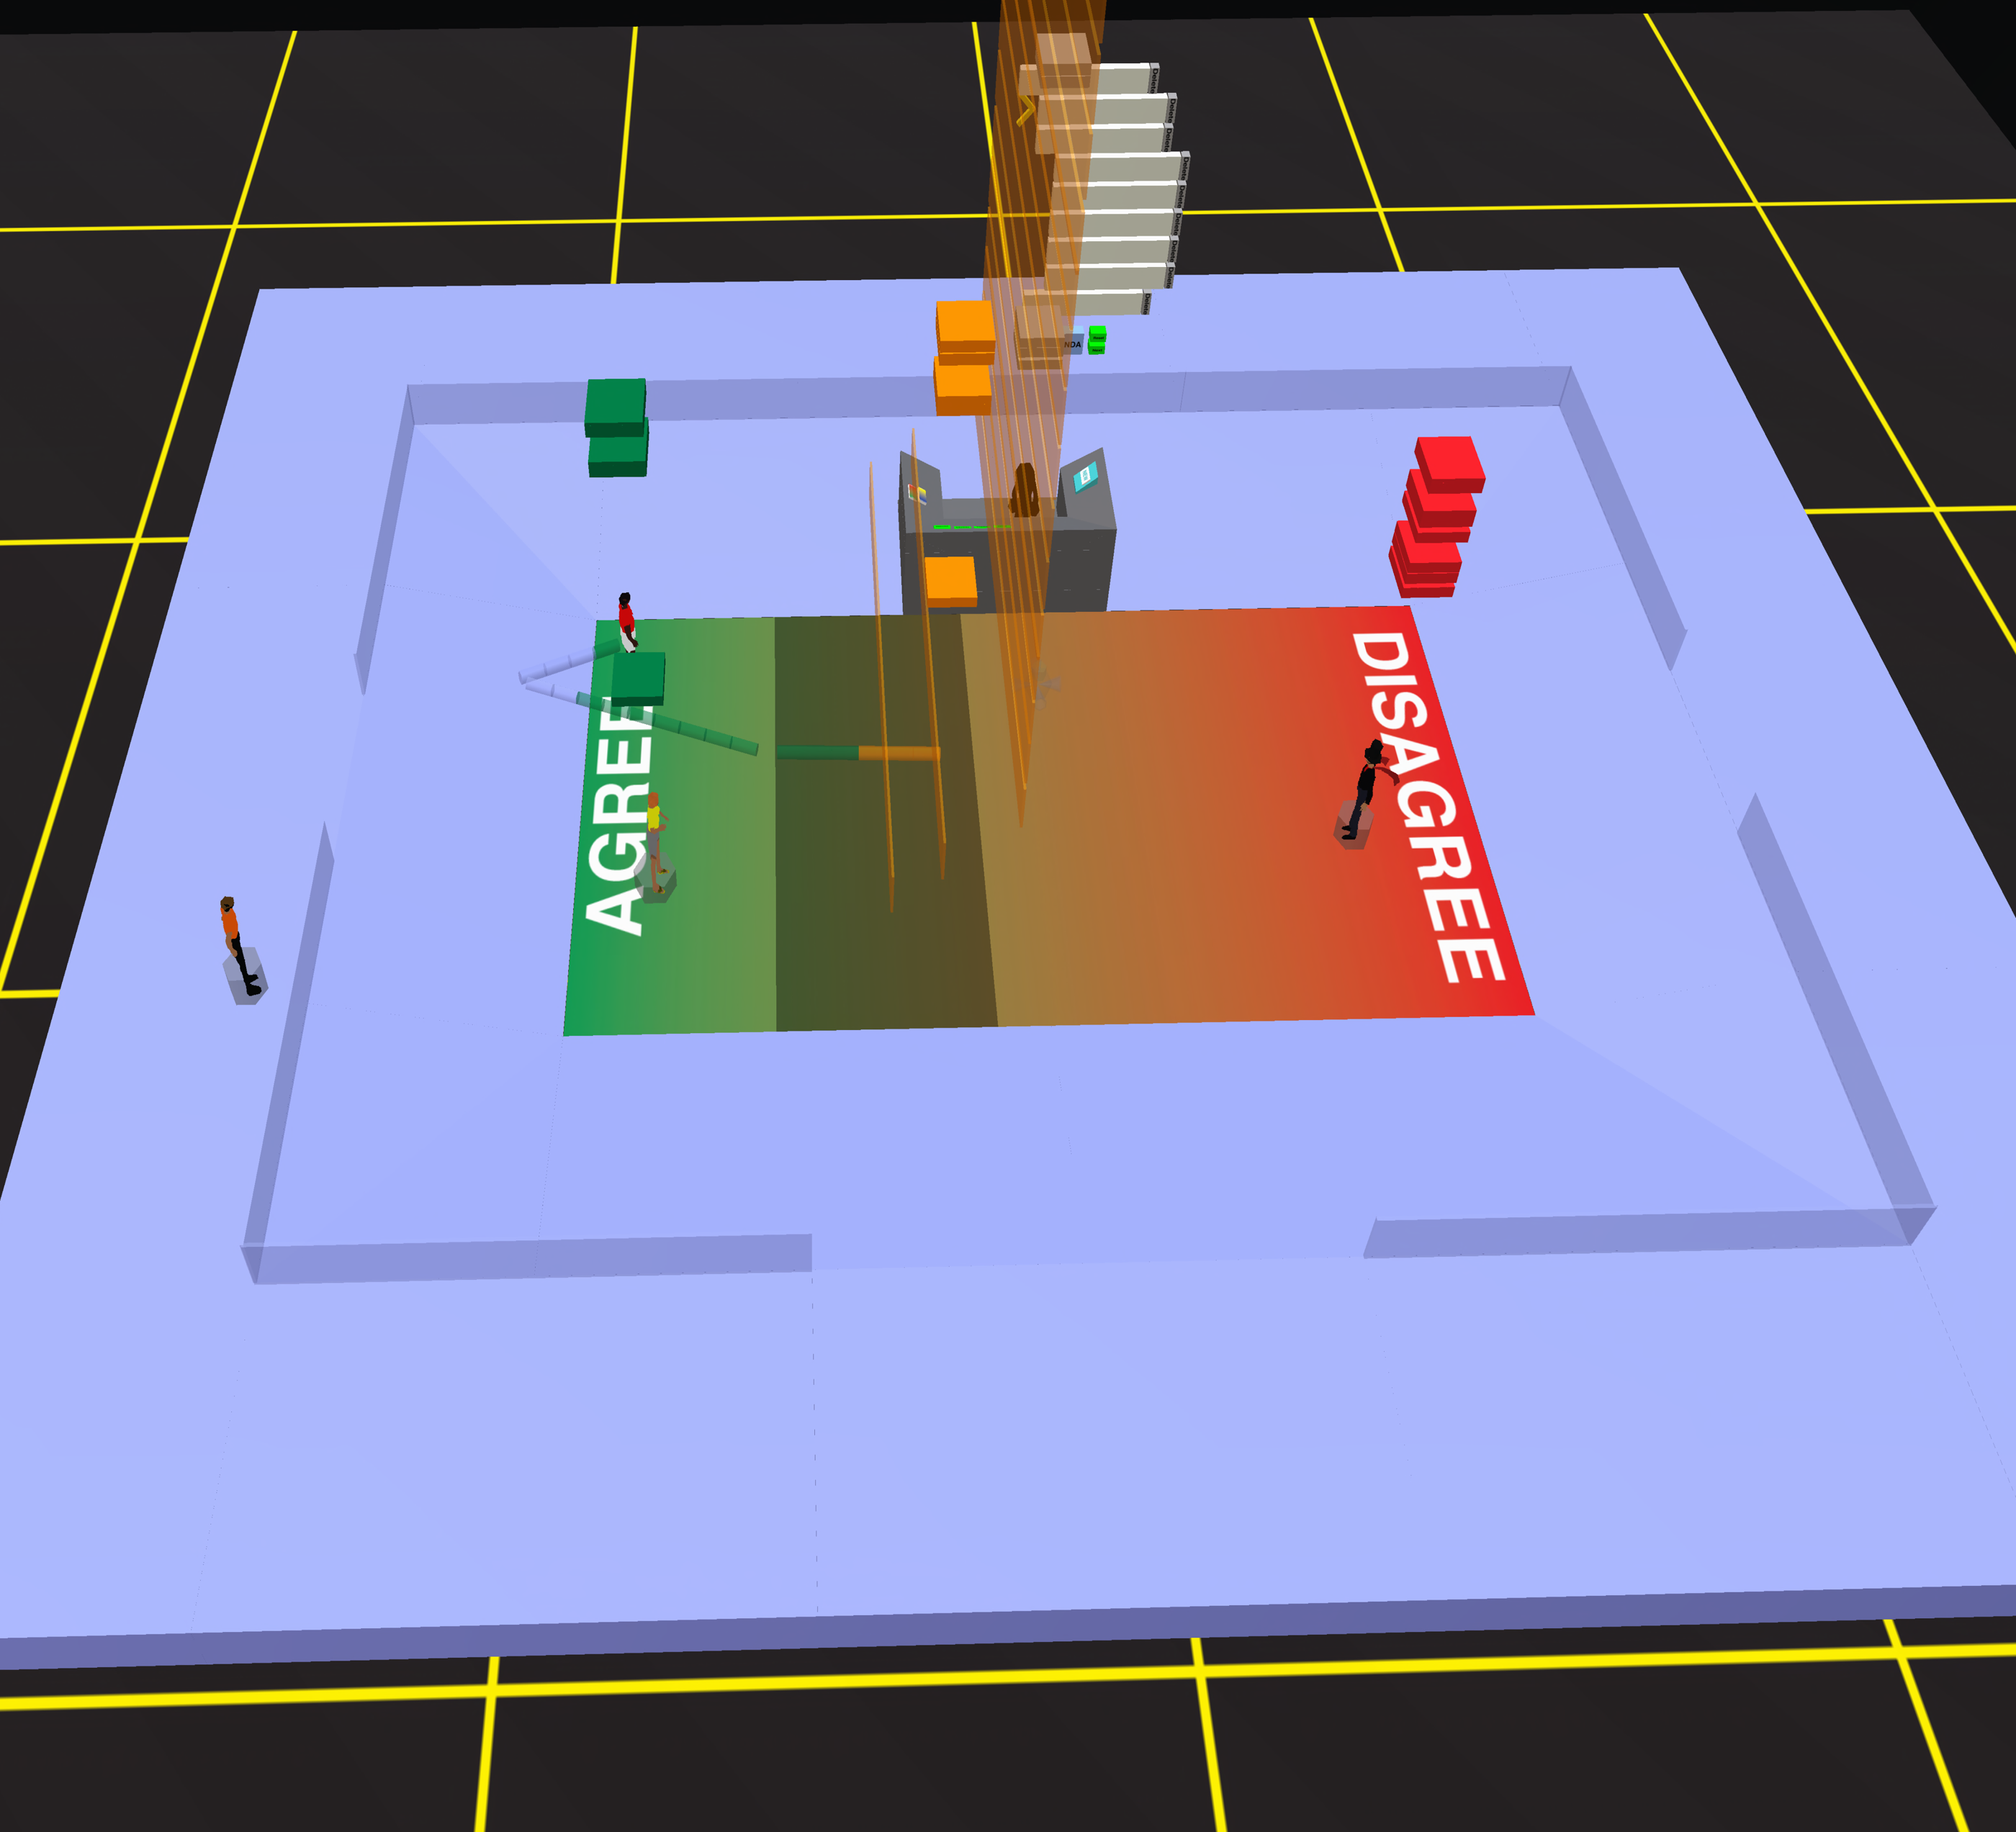
\includegraphics{figures/information-space-iso-overview.png}
	\caption{An isometric overview of the \emph{Information Space} with all the visualization components turned on.}
	\label{fig:information_space_overview}
\end{figure*}

Core to the aesthetics of this space is a belief that virtual worlds have distinctly different properties from the physical world, and so a meeting space in a virtual world should not only look different, but our traditional models of people sitting around a table are not necessarily the most effective environment. The subtle signals that guide our interactions in that context are missing in a virtual world context, even if we're represented by avatars. With this design, I focus on creating new ways for people to represent their attitudes and emotions in a mode that is easily effected and understood by others.



\subsection{Space Design}

The space is divided into four major zones. The main area is like a traditional sports field with end zones labeled ``agree'' and ``disagree''. It provides a space for people to position their avatars on a continuum to show their attitudes about the issue under discussion. The fluid self-arrangement of people within this space based on their opinions provides a literal basis for seeing where someone is coming from and the status of the group's attempt to reach consensus. A single-axis continuum is used so that multiple people can easily be at the same continuum position without displacing each other.

Of course, not everyone always wants to reveal their opinion about the issue at hand. Surrounding the main agree/disagree field is an area for people to stand who want to participate in the discussion without putting their avatar on the continuum. Still further from the field is an observation area for people who want to be present, but not participating. Finally, there is a platform for the moderator with controls to manage properties about the space itself. This layout is shown in figure \ref{fig:information_space_layout}. For the sake of simplicity, most examples in this chapter will focus on the Agree/Disagree continuum, but the implications of other floor types (for instance a process oriented Keep Talking/Move On field) will be discussed later. This spatial approach is a powerful organizational metaphor because it both relies on our knowledge of the meanings of position relative to other people in physical spaces \citep{Yee:2007cl} and the metaphors inherent to interactions in a spatial environment. \citep{lakoff_metaphors_1980}

The Agree/Disagree floor is only one potential floor design. Although it makes for a good thought experiment and it will be used for much of this section, its actual utility is limited. Few meetings are sufficiently organized for this approach to be effective. Even with a strong moderator who makes clear exactly what issue avatar's positions are agreeing or disagreeing with it can at times be ambiguous. There are a number of other options for floor designs that are more generally useful.

\begin{marginfigure}
	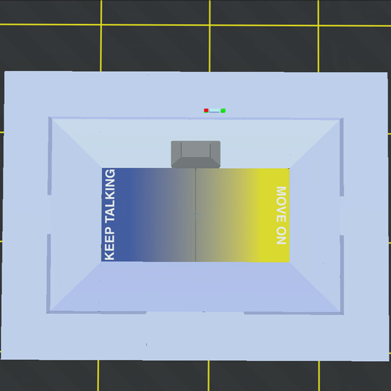
\includegraphics{figures/keep_talking_from_above.png}
	\caption{A view of the keep talking / move on space from above.}
	\label{fig:keep_talking_floor}
\end{marginfigure}

The primary alternative is a Keep Talking/Move On floor. This floor addresses the need for meeting participants to be able to express when they think the group as a whole should change to a new discussion topic. In much the same way that Robert's Rules of Order \citep{RobertIII:2000tq} is a process that is focused on how time is spent, using the Keep Talking/Move On floor is a way of actively expressing your desire to move on or keep talking about an issue and for others to passively judge the interests of the group, even if a more formal structure is not in place. This is a generic issue, and is one that can be particularly hard to resolve in medium-sized groups. Participants might not want to speak up and say that they want to move on, but if they had a non-verbal way to express their desire to move on (and gauge others' reactions) meetings might spend less time on topics that they didn't need to.





Although these are the only two floor designs that are currently implemented, there is potential in other kinds of floors. Floors with a few multiple choice options make it easy to hold straw polls. A calendar display could be used to show preferred dates for an event. Floors could be used for setting up speaking queues, as well, dividing the audience between those who are waiting to say something, those who are speaking, and those who don't have anything to say. Multi-variate floors are also possible, although there isn't a nice way to let multiple avatars stand at the same point in the space in the same way that you can in single variable floors like Agree/Disagree.

\begin{marginfigure}
	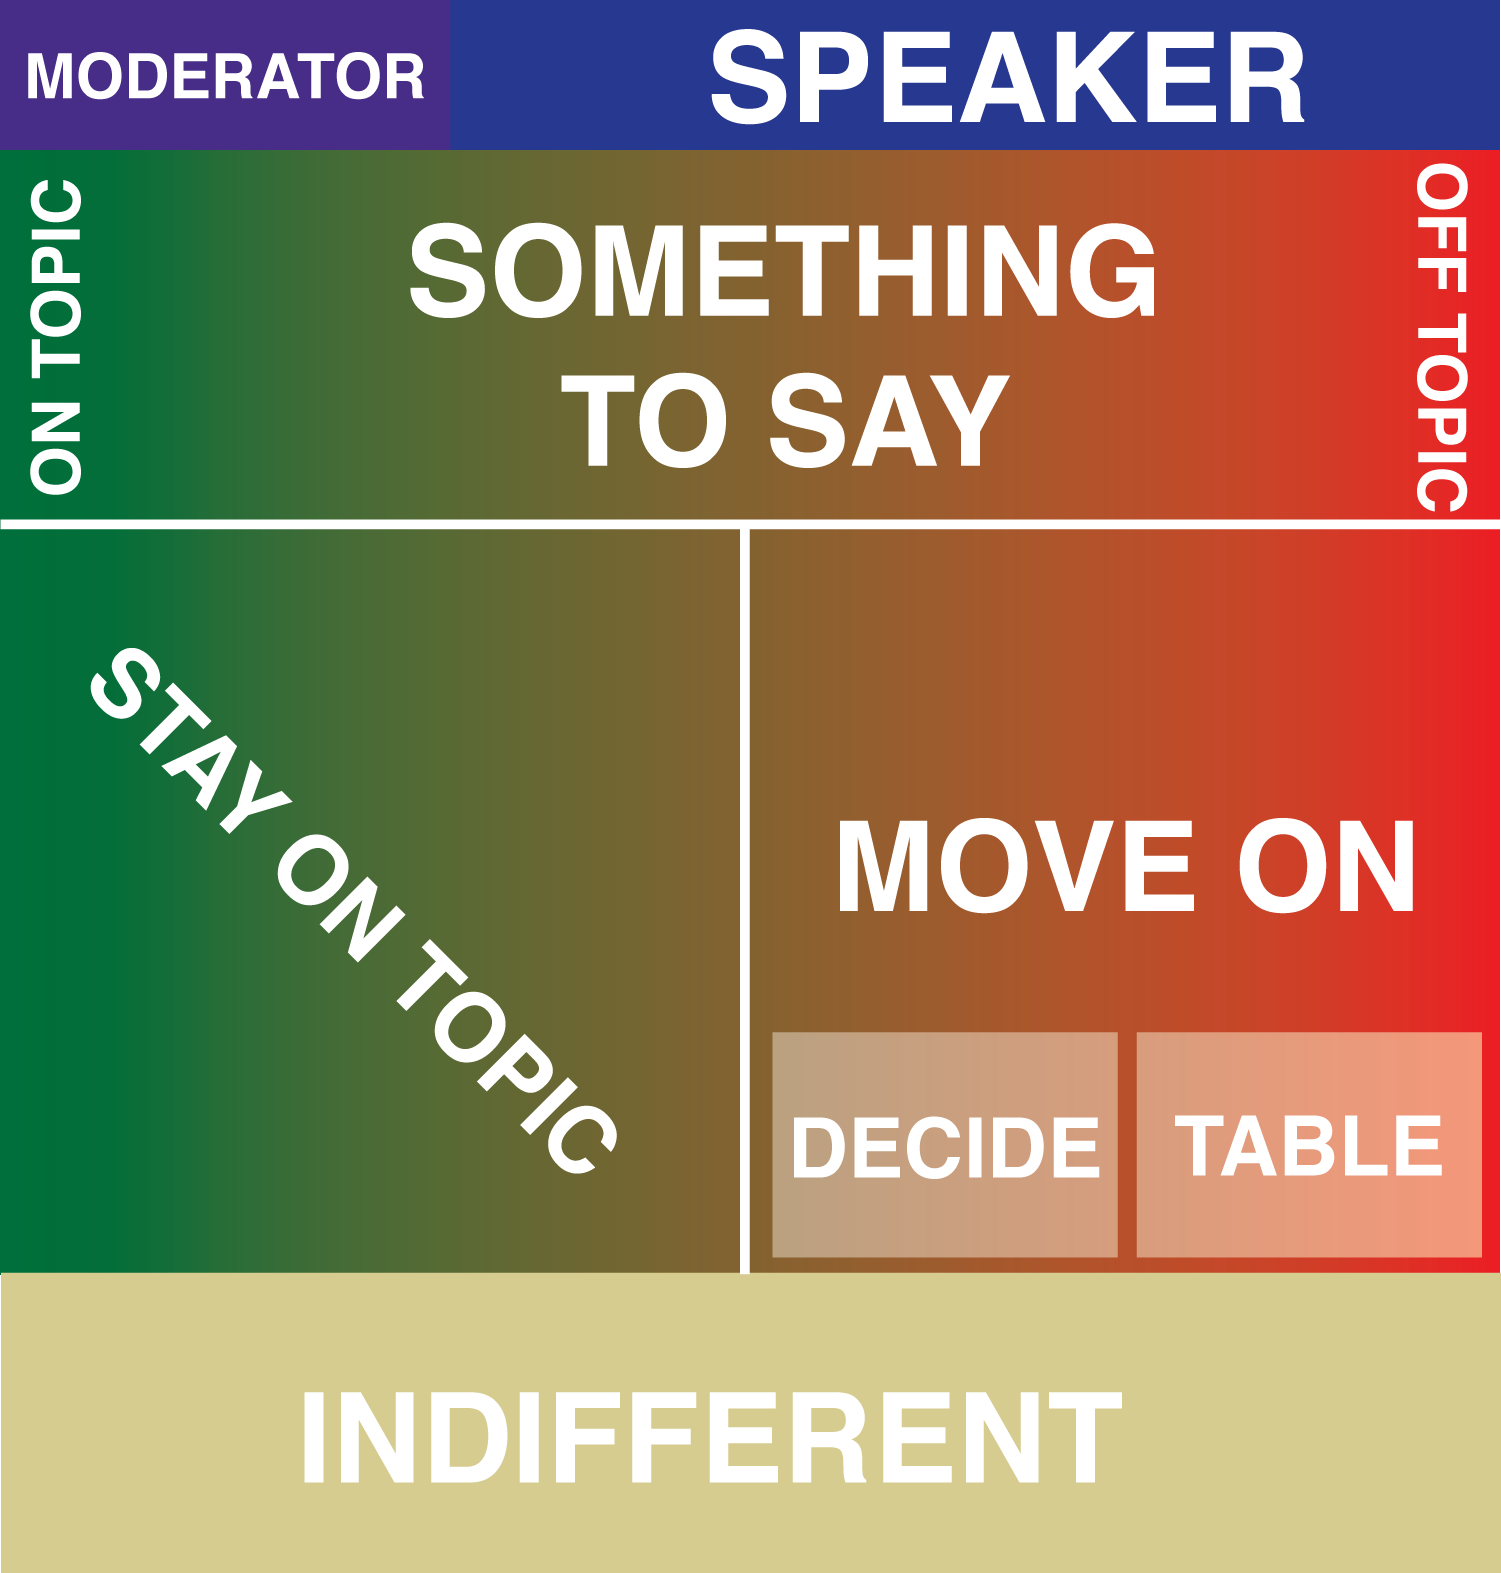
\includegraphics{figures/agree-disagree-redux-floor.png}
	\caption{An early floor design from the first \emph{Information Spaces} prototype. Far more complex than subsequent designs, this approach sought to support a much wider range of non-verbal actions. Ultimately, the design shifted to create some of these spaces in less explicit ways and to expect less frequent movement on the part of participants; this floor implied constant shuffling around as speakers changed and queued to speak.}
	\label{fig:agree_disagree_initia_design}
\end{marginfigure}


\begin{figure*}[t]
	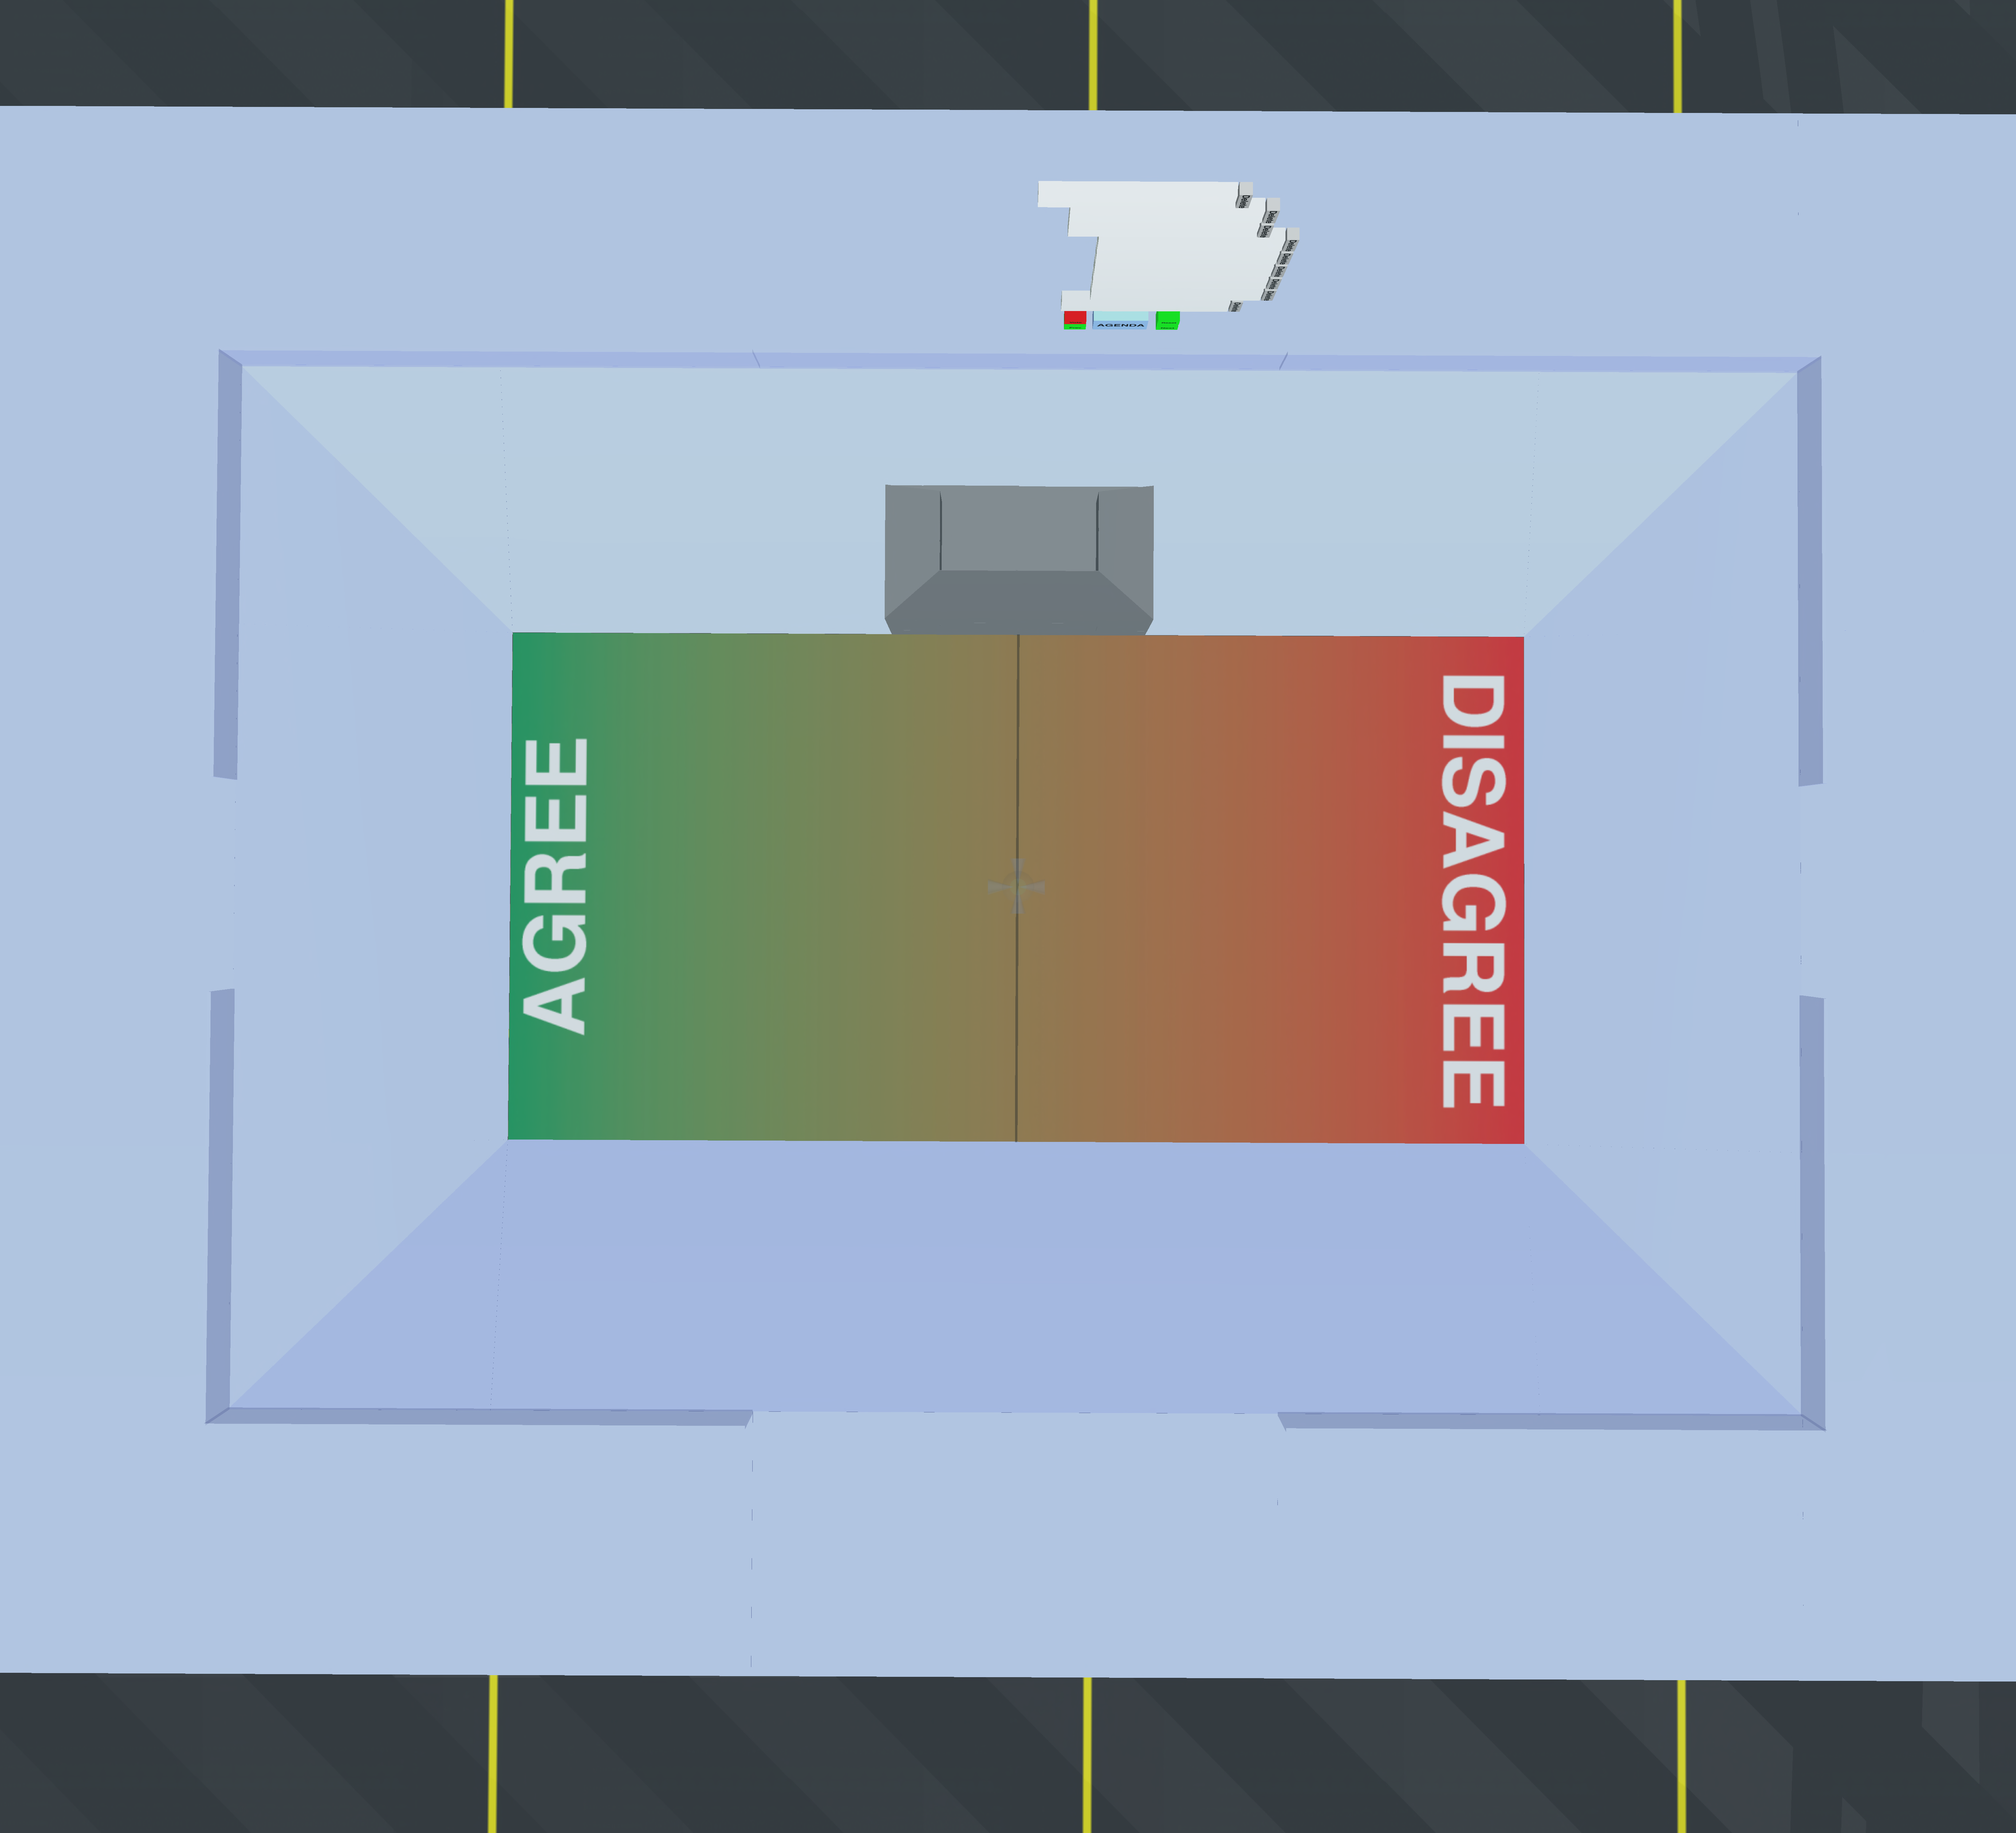
\includegraphics{figures/layout.png}
	\caption{A top-down view of the space, to illustrate its different zones.}
	\label{fig:information_space_layout}
\end{figure*}

Because the space is divided into socially meaningful regions, the most important information we can visualize about someone's position is how long they've been somewhere and where they last came from. When an avatar pauses for a while, a transparent column will slowly rise out of the ground. I call these columns ``dwell indicators.'' If they move, the column will slowly shrink and eventually disappear. In this way, avatars leave a temporary mark on the space with their presence, and other people can use this signal to better understand what their position means. Someone who has been standing on the agree side of the field for the entire discussion is quite different from someone who just arrived there; this approach distinguishes those meanings visually. A dwell indicator is shown in figure \ref{fig:information_space_dwell}.

As an avatar moves around this space, their path is drawn behind them. This helps meeting participants understand how an avatar arrived at their current position. In particular, it fits well with the dwell indicators; when an avatar who has been standing somewhere for a while (as shown by the dwell indicator) moves to a new position, their old dwell indicator will start to shrink and a line is drawn between their old position to their new position. This connects the two dwell indicators and shows how long the avatar was in their previous position, and how recently they moved. In the case of the agree/disagree floor, this would show that someone who perhaps had long been against a particular proposal had changed their mind. This is the kind of behavior that this space seeks to visually emphasize because it's socially meaningful but is otherwise hard to convey non-verbally. A position history trace is shown in figure \ref{fig:information_space_traces}.

\begin{figure*}[tp]
	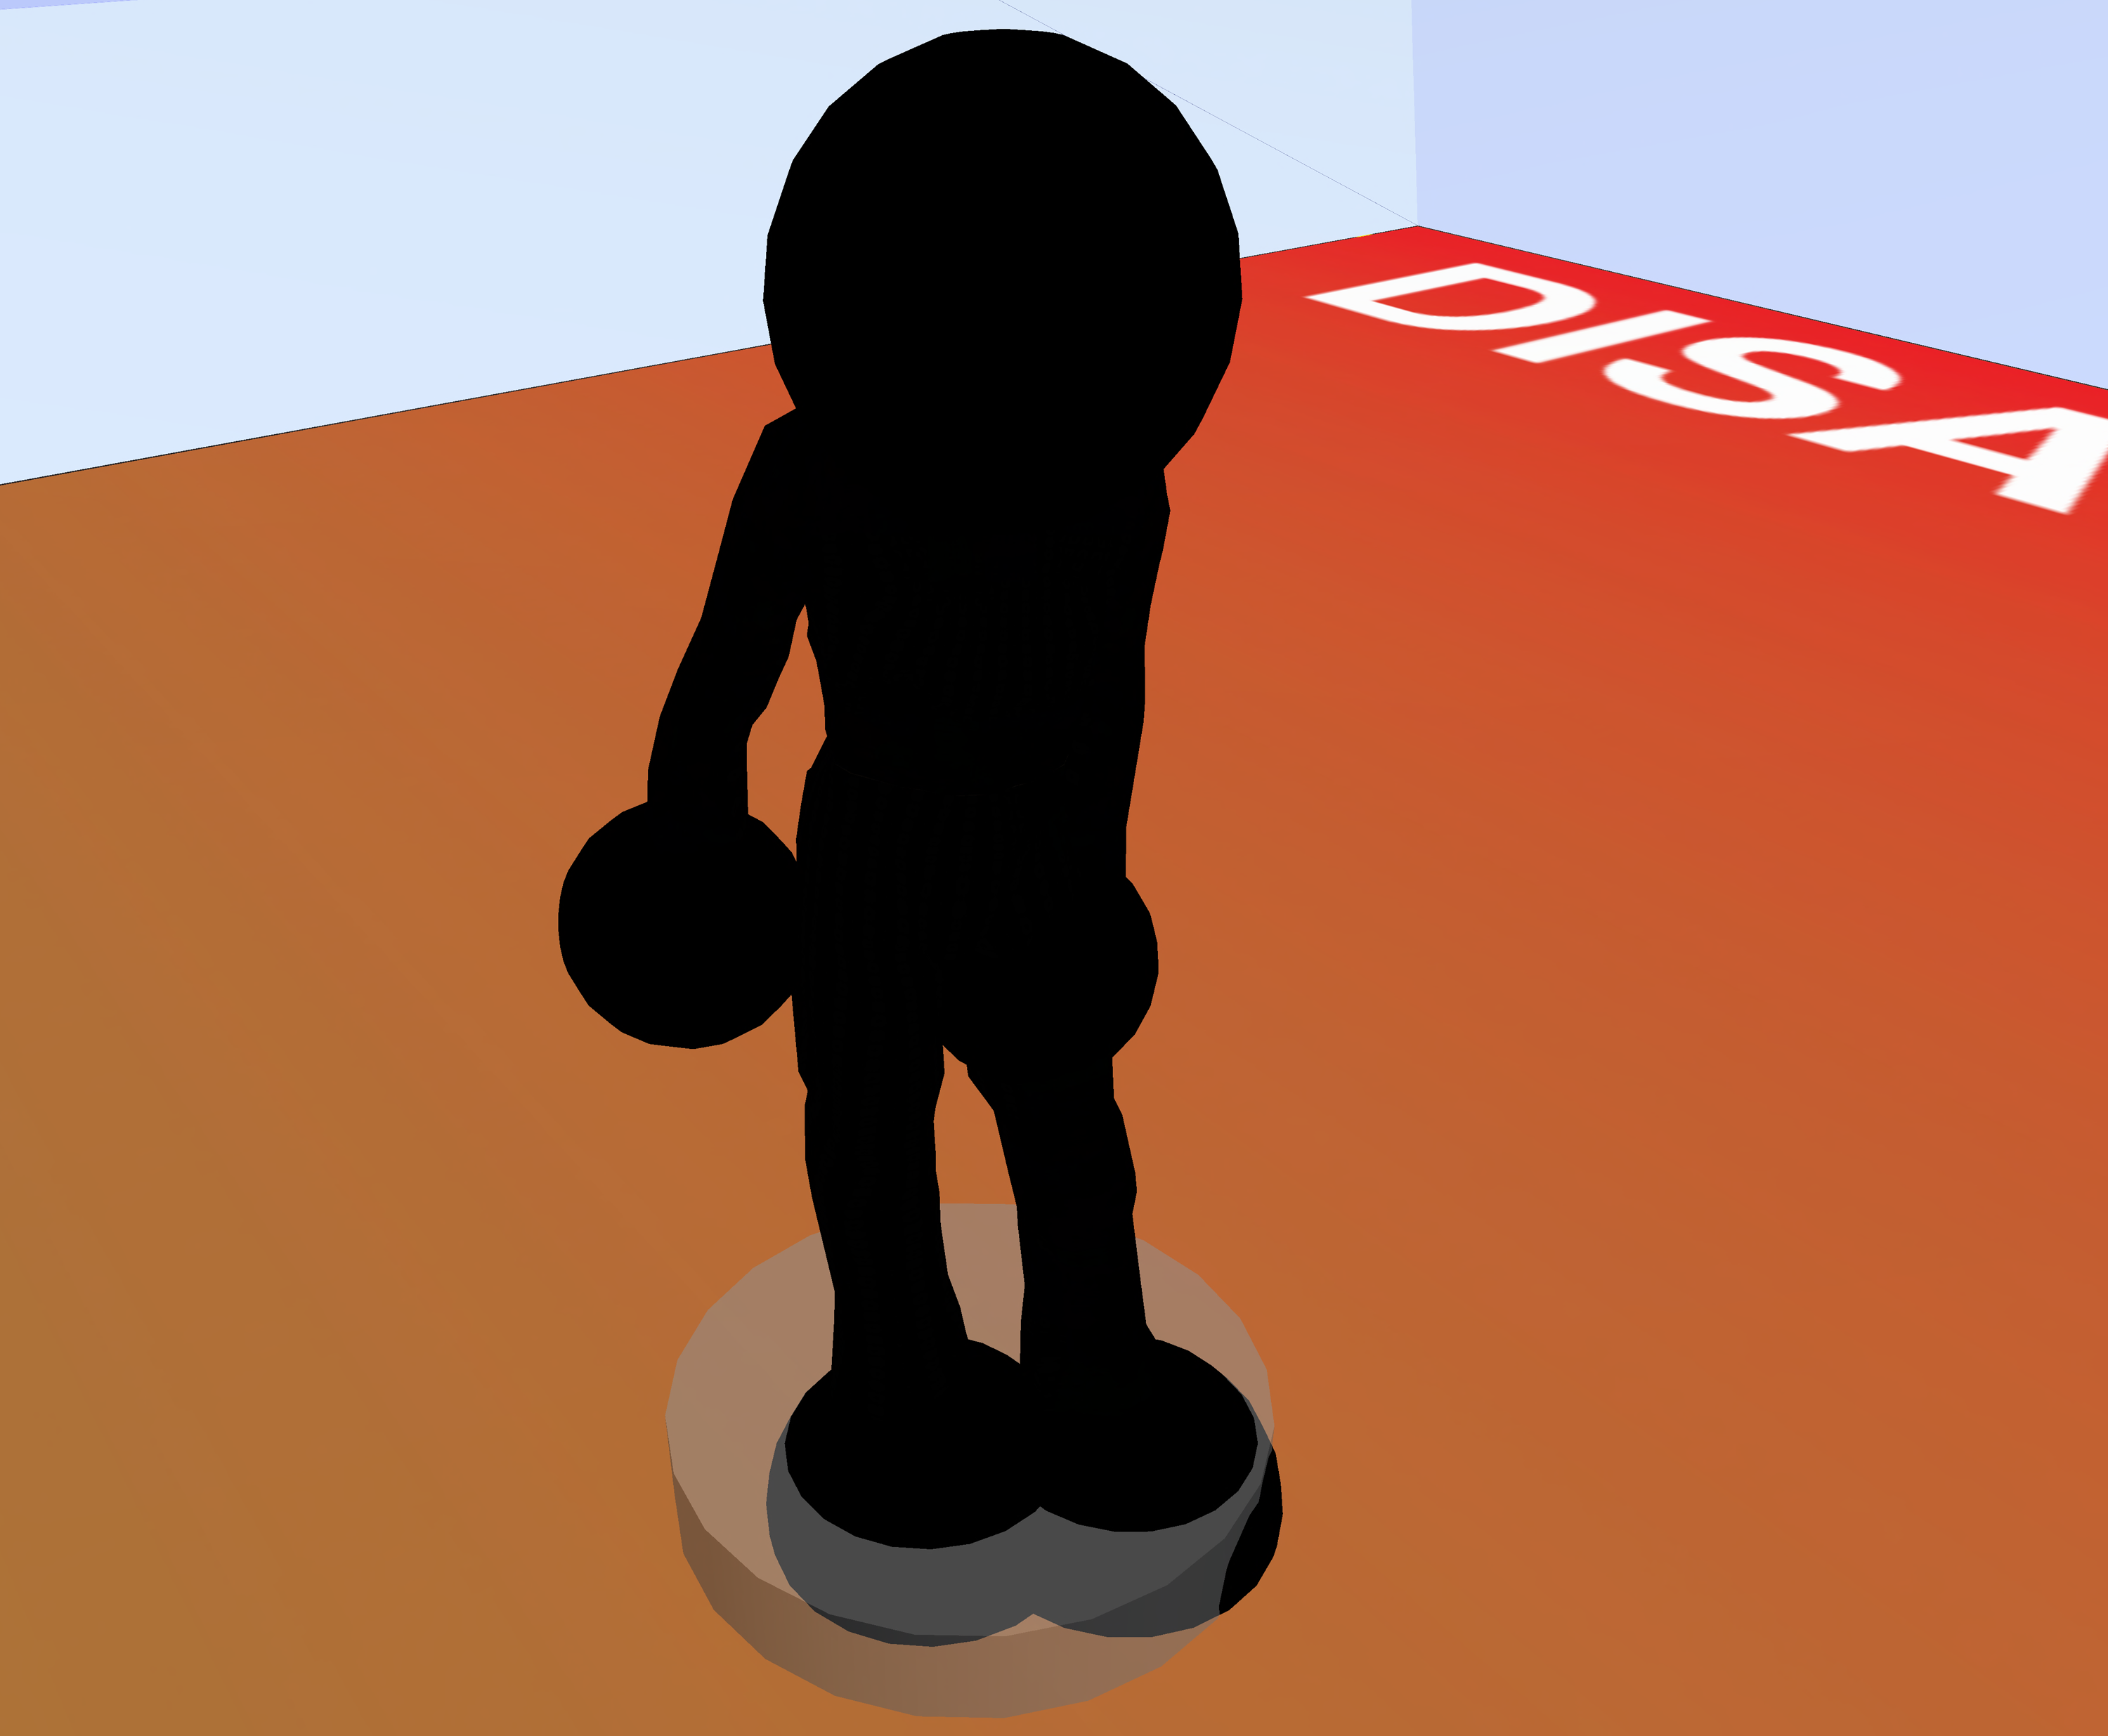
\includegraphics{figures/dwell-crop-lower.png}
	\caption{An avatar with a dwell indicator growing slowly at its feet.}
	\label{fig:information_space_dwell}
\end{figure*}

\begin{figure*}[tp]
	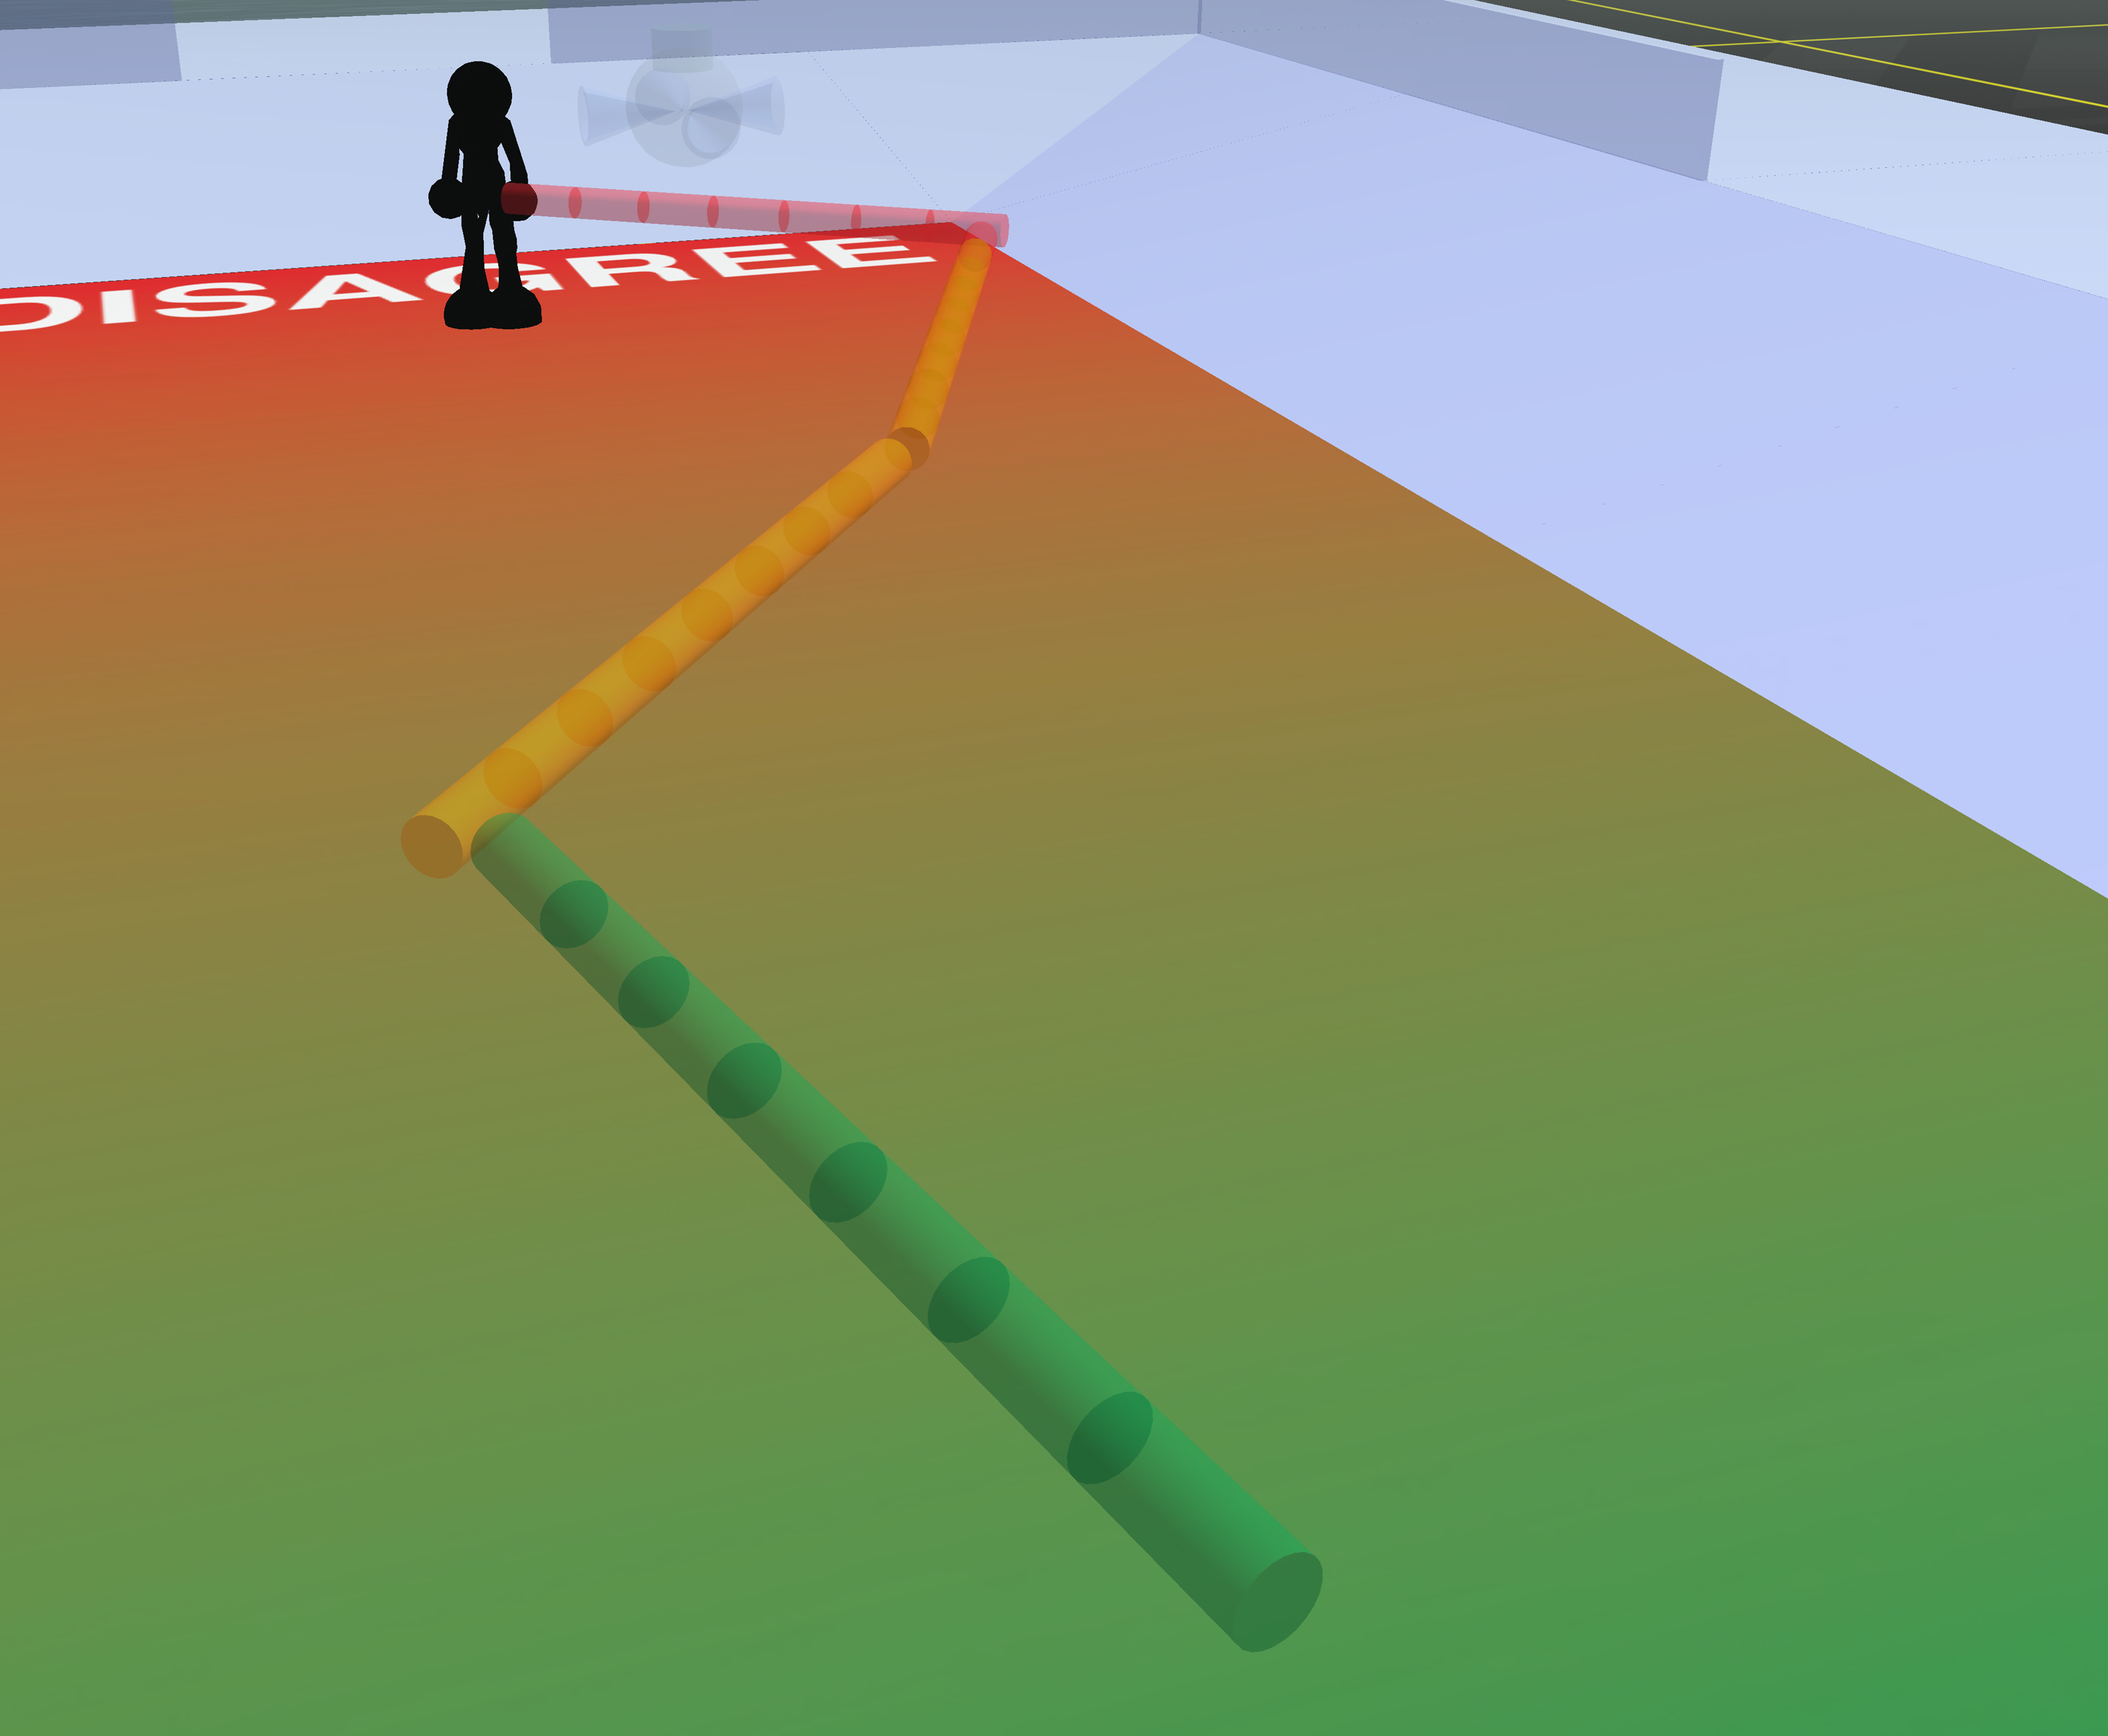
\includegraphics{figures/traces-lower.png}
	\caption{An avatar after moving from the agree side to the disagree side. The position history shows the avatar's path, and is colored according to the area in the space they were in.}
	\label{fig:information_space_traces}
\end{figure*}

\begin{figure*}[tp]
	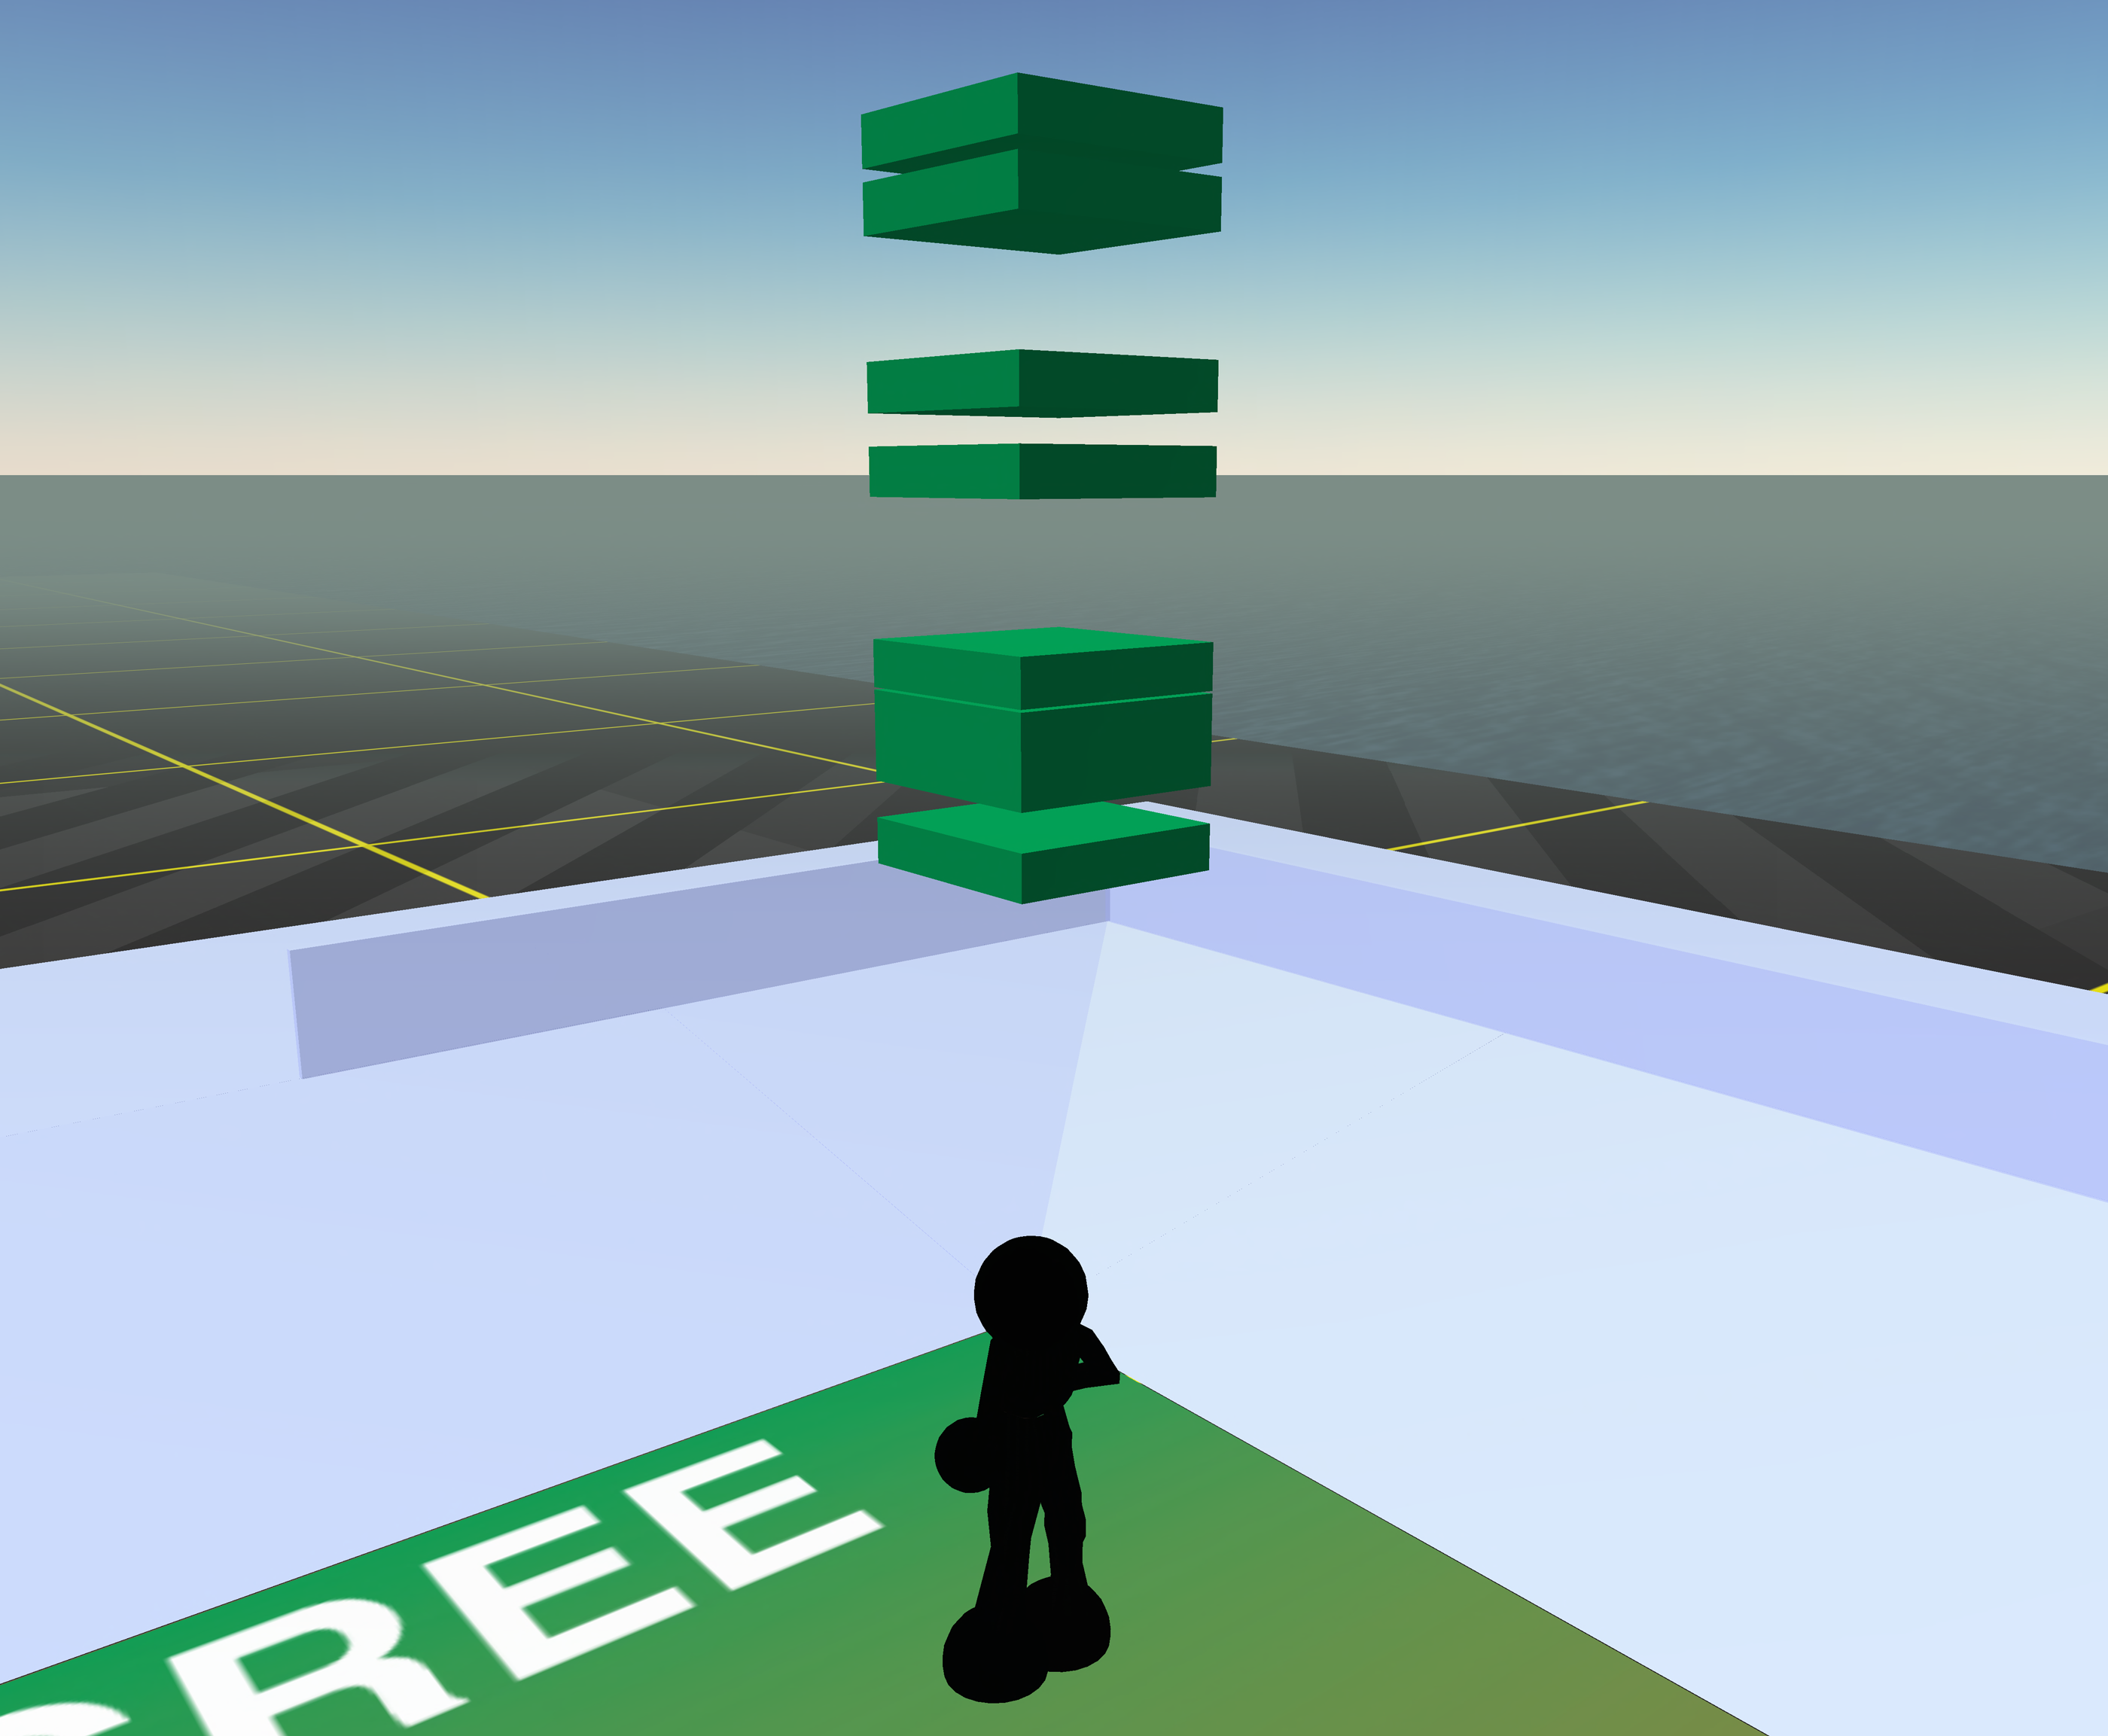
\includegraphics{figures/chat-history-lower.png}
	\caption{Chat messages rising above the head of the speaker.}
	\label{fig:information_space_chat}
\end{figure*}

The space also records typed contributions in text boxes that appear above the speaker's head and then rise slowly. This creates a visualization of chat over the course of the meeting, displaying what was said, when it was said, and where in the room the avatar was when they said it. \citep{DiMicco:2007ie} In aggregate, it also shows that patterns of conversation of the course of the meeting. Much like the conversation visualization work discussed in earlier chapters, this allows participants to be self-reflective about the dynamics of the meeting as it occurs. By making objects appear in the space itself, it foregrounds these issues and makes imbalances in participation harder to avoid. Because the boxes contain the text itself, it is also possible for participants to zoom in on text messages and view the conversation within its spatial context---which is lost in a text-only transcript of the meeting).

Finally, the floor of the agree/disagree field displays the current average vote (by moving side to side along the floor), as well as its deviation (by growing wider or thinner). Like chat messages, a representation of the group's collective view also floats up into the sky. These bars provide more context about the overall feeling of the avatars in the space over time, showing aggregate views of avatar movement. Furthermore, the history of the average position separates historical chat messages based on which side of the average the message came from. This helps contextualize the chat messages as well. For instance, it is easy to tell if a talkative participant was way out of line relative to the group consensus.

\begin{figure*}[t]
	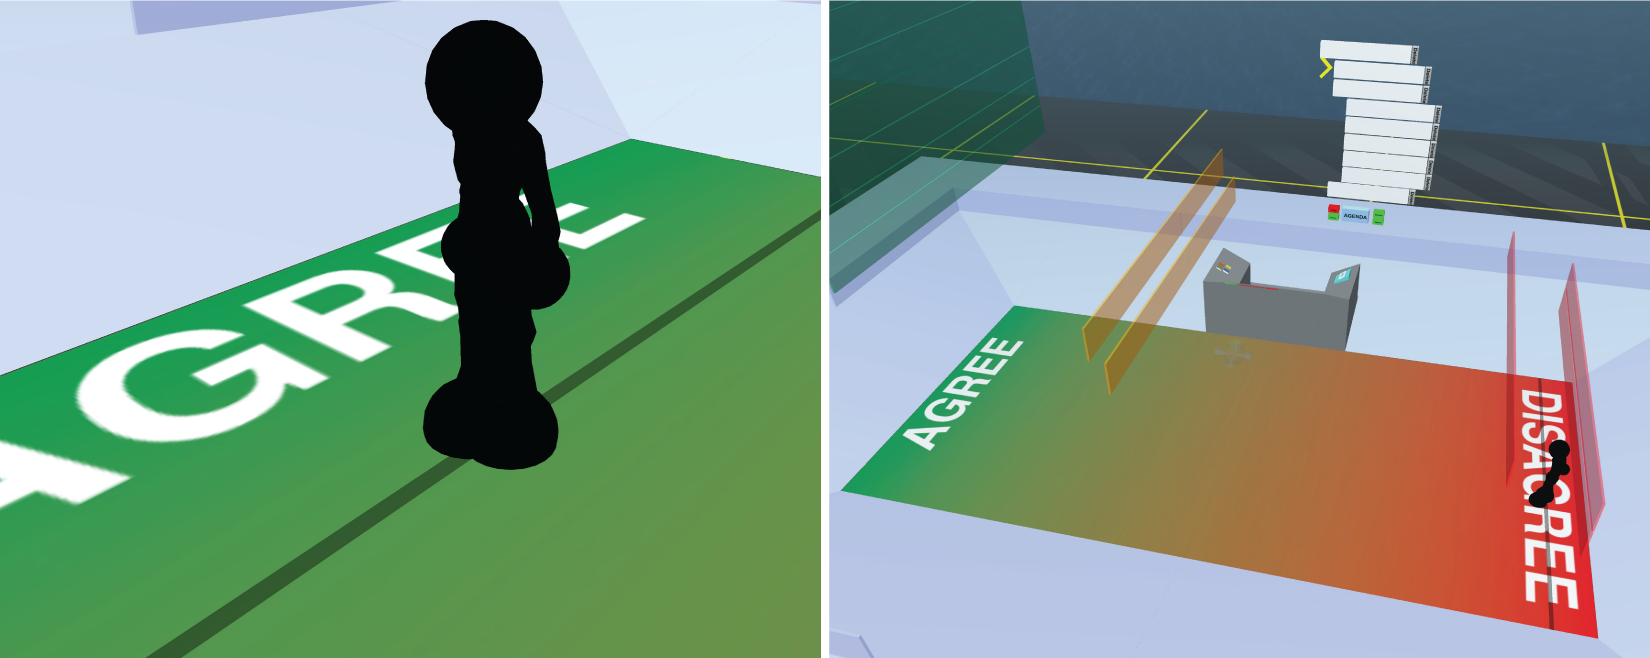
\includegraphics{figures/average+history.png}
	\caption{Left: A view of the floor with a line showing the current average vote. Right: In the space above the meeting room, long bars float slowly up to represent the history of the average vote over time.}
	\label{fig:information_space_average_history}
\end{figure*}

\subsection{Discussion Tools}

During the process of developing the Agree/Disagree space, it became clear that there were a number of other common events in meetings that could be easily supported with applications. From an application design perspective, the main benefit of working in a virtual world is that it's easy to export information into shared conceptual space of the meeting room. This is a common practice in face-to-face meetings in the form of slideshows, keeping live agendas on a projected screen. It's particularly prevalent in group design practice, in which a fluid and grounded conversation about ideas is valuable. \citep{Dwyer:2005uj} It's easy to facilitate this process by creating objects in the virtual world that hold information. The kinds of information that are easily represented in Second Life and the challenges of working without any familiar UI widgets or metaphors limit the overall efficacy of these applications, but they are interesting first steps in building specific objects that offer functionality that can further customize the meeting room experience. Unlike in physical rooms, which are largely limited by the number of projectors available to augment the space with information, virtual spaces have many more opportunities to customize the experience.

Often, meetings involve some sort of distribution of tasks. This process is usually an elaborate (and sometimes unspoken) negotiation between who has time to do a task, is interested in getting it done, and the skills necessary to complete it. This application addresses availability. When a task is going to be assigned, the meeting moderator can press a button on meeting dashboard and a small pyramid will appear. (Figure \ref{fig:information_space_todo}) Text can be stored in the pyramid by typing `/todo ' followed by the text of the task. Anyone can then click on the task to claim it. Claimed tasks spin slowly above the head of the claimant. As an avatar with claimed tasks moves around, the tasks follow above their head. Tasks also have buttons on them, allowing the owner to release them (so they can be claimed by someone else) or delete them outright. The vision for this particular application is that tasks would also export from

The task objects serve as visual reminders of who in the group has already accepted tasks and who hasn't. Much like visualizing chat can encourage participation from people who are participating below average, this can serve a similar role. Task objects also operate metaphorically - by staying above an avatars head, they rely on the metaphor of tasks ``hanging over us.'' \citep{lakoff_metaphors_1980} This kind of allusion doesn't work nearly as well face to face. Although you could hand out note cards with tasks on them, it would not have the same metaphorical resonance as the virtual approach does.


\begin{figure*}[tp]
	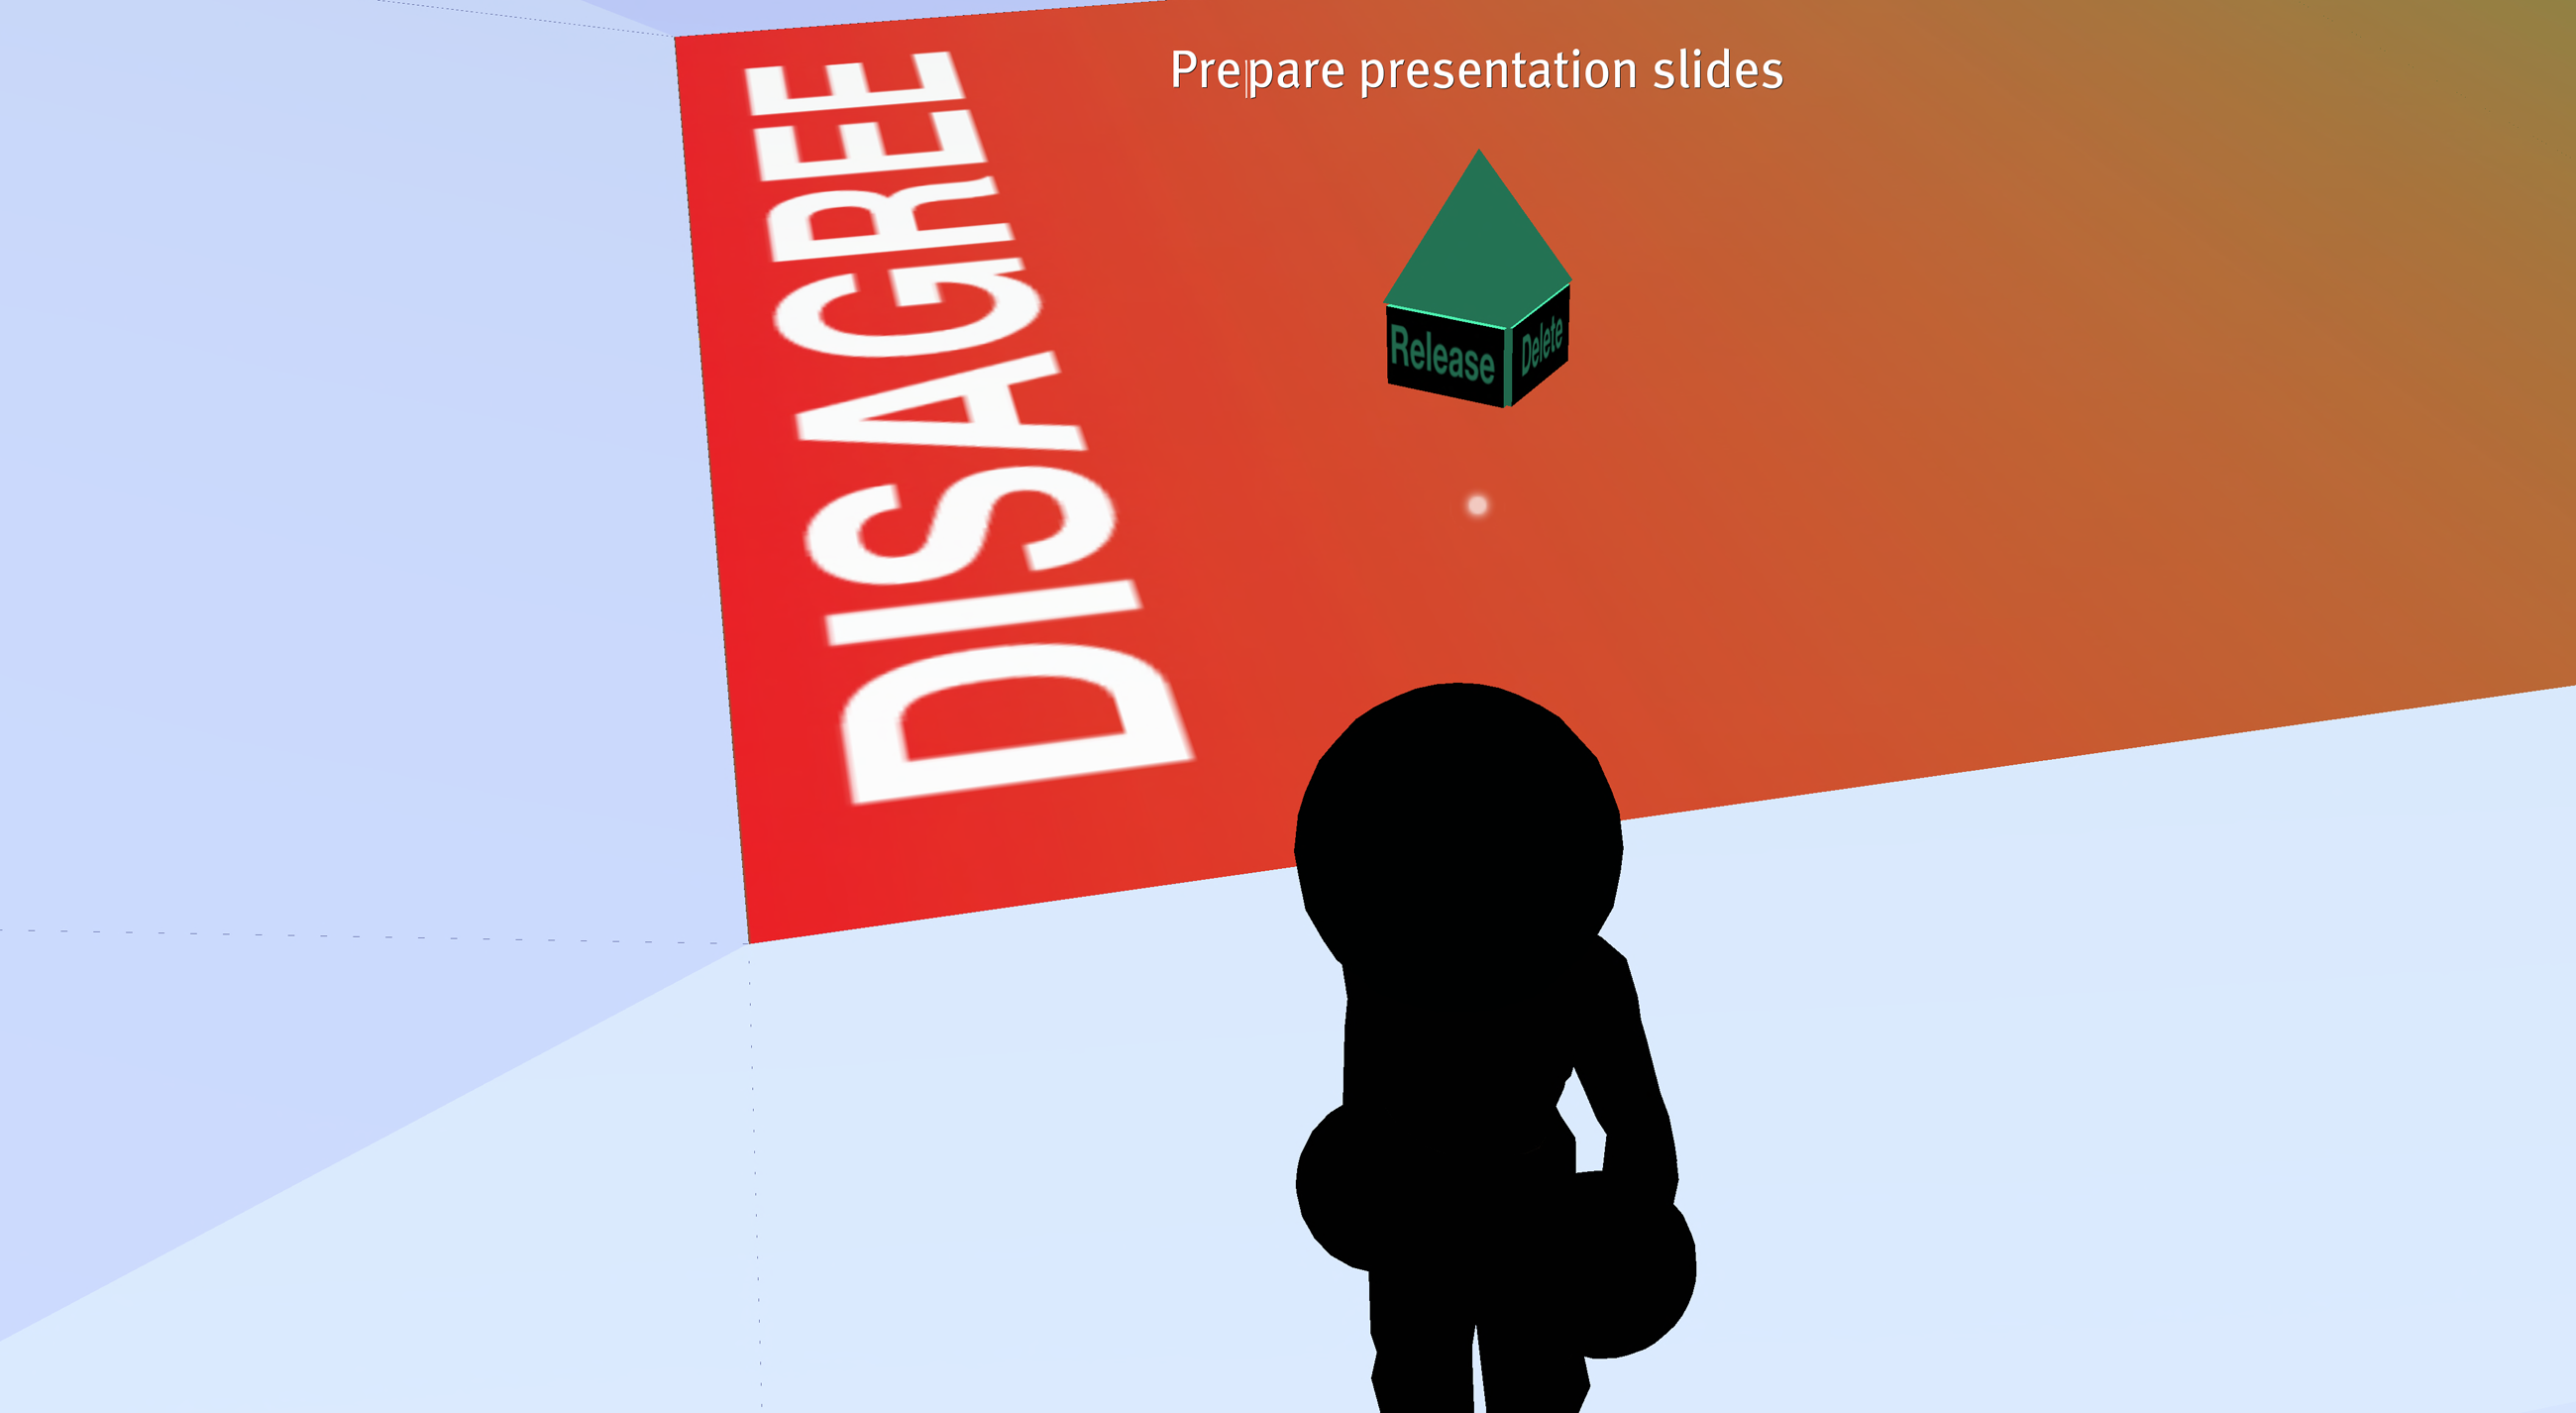
\includegraphics{figures/todo.png}
	\caption{A todo pyramid floating above an avatar's head. Buttons below the pyramid provide a mechanism for deleting the todo or releasing it so someone else can claim it.}
	\label{fig:information_space_todo}
\end{figure*}


Having a representation of the agenda in a meeting space can be a helpful way to both remind people of the what the current status of the meeting is. (Figure \ref{fig:information_space_agenda}) This tool takes a note card object in Second Life and represents it as a hierarchical listing in the meeting room. The moderator can move a pointer between agenda items to indicate which one is currently under discussion. The system also has a voting mode, in which agenda items also act as buttons that accumulate votes. By default, the voting system operates using an approval voting in which a single avatar can vote for as many options as they want, but cannot vote for a single option more than once. As votes accumulate, the color of the item changes to quickly show which items are the most popular. In the spirit of configurable spaces, there are a number of ways the voting system can be reconfigured. Votes can either accumulate secretly until the end of the vote, or be shown as they are received. Voting can be approval or traditional first-past-the-post. Ballots can either be public or private. Depending on the kind of vote being held, different configurations would be appropriate. Although this doesn't offer nearly the flexibility of a system like Selectricity \citep{Hill:2006vw}, embedding the voting in the virtual space serves as a visual reminder to past votes.
 


\begin{figure*}[tp]
	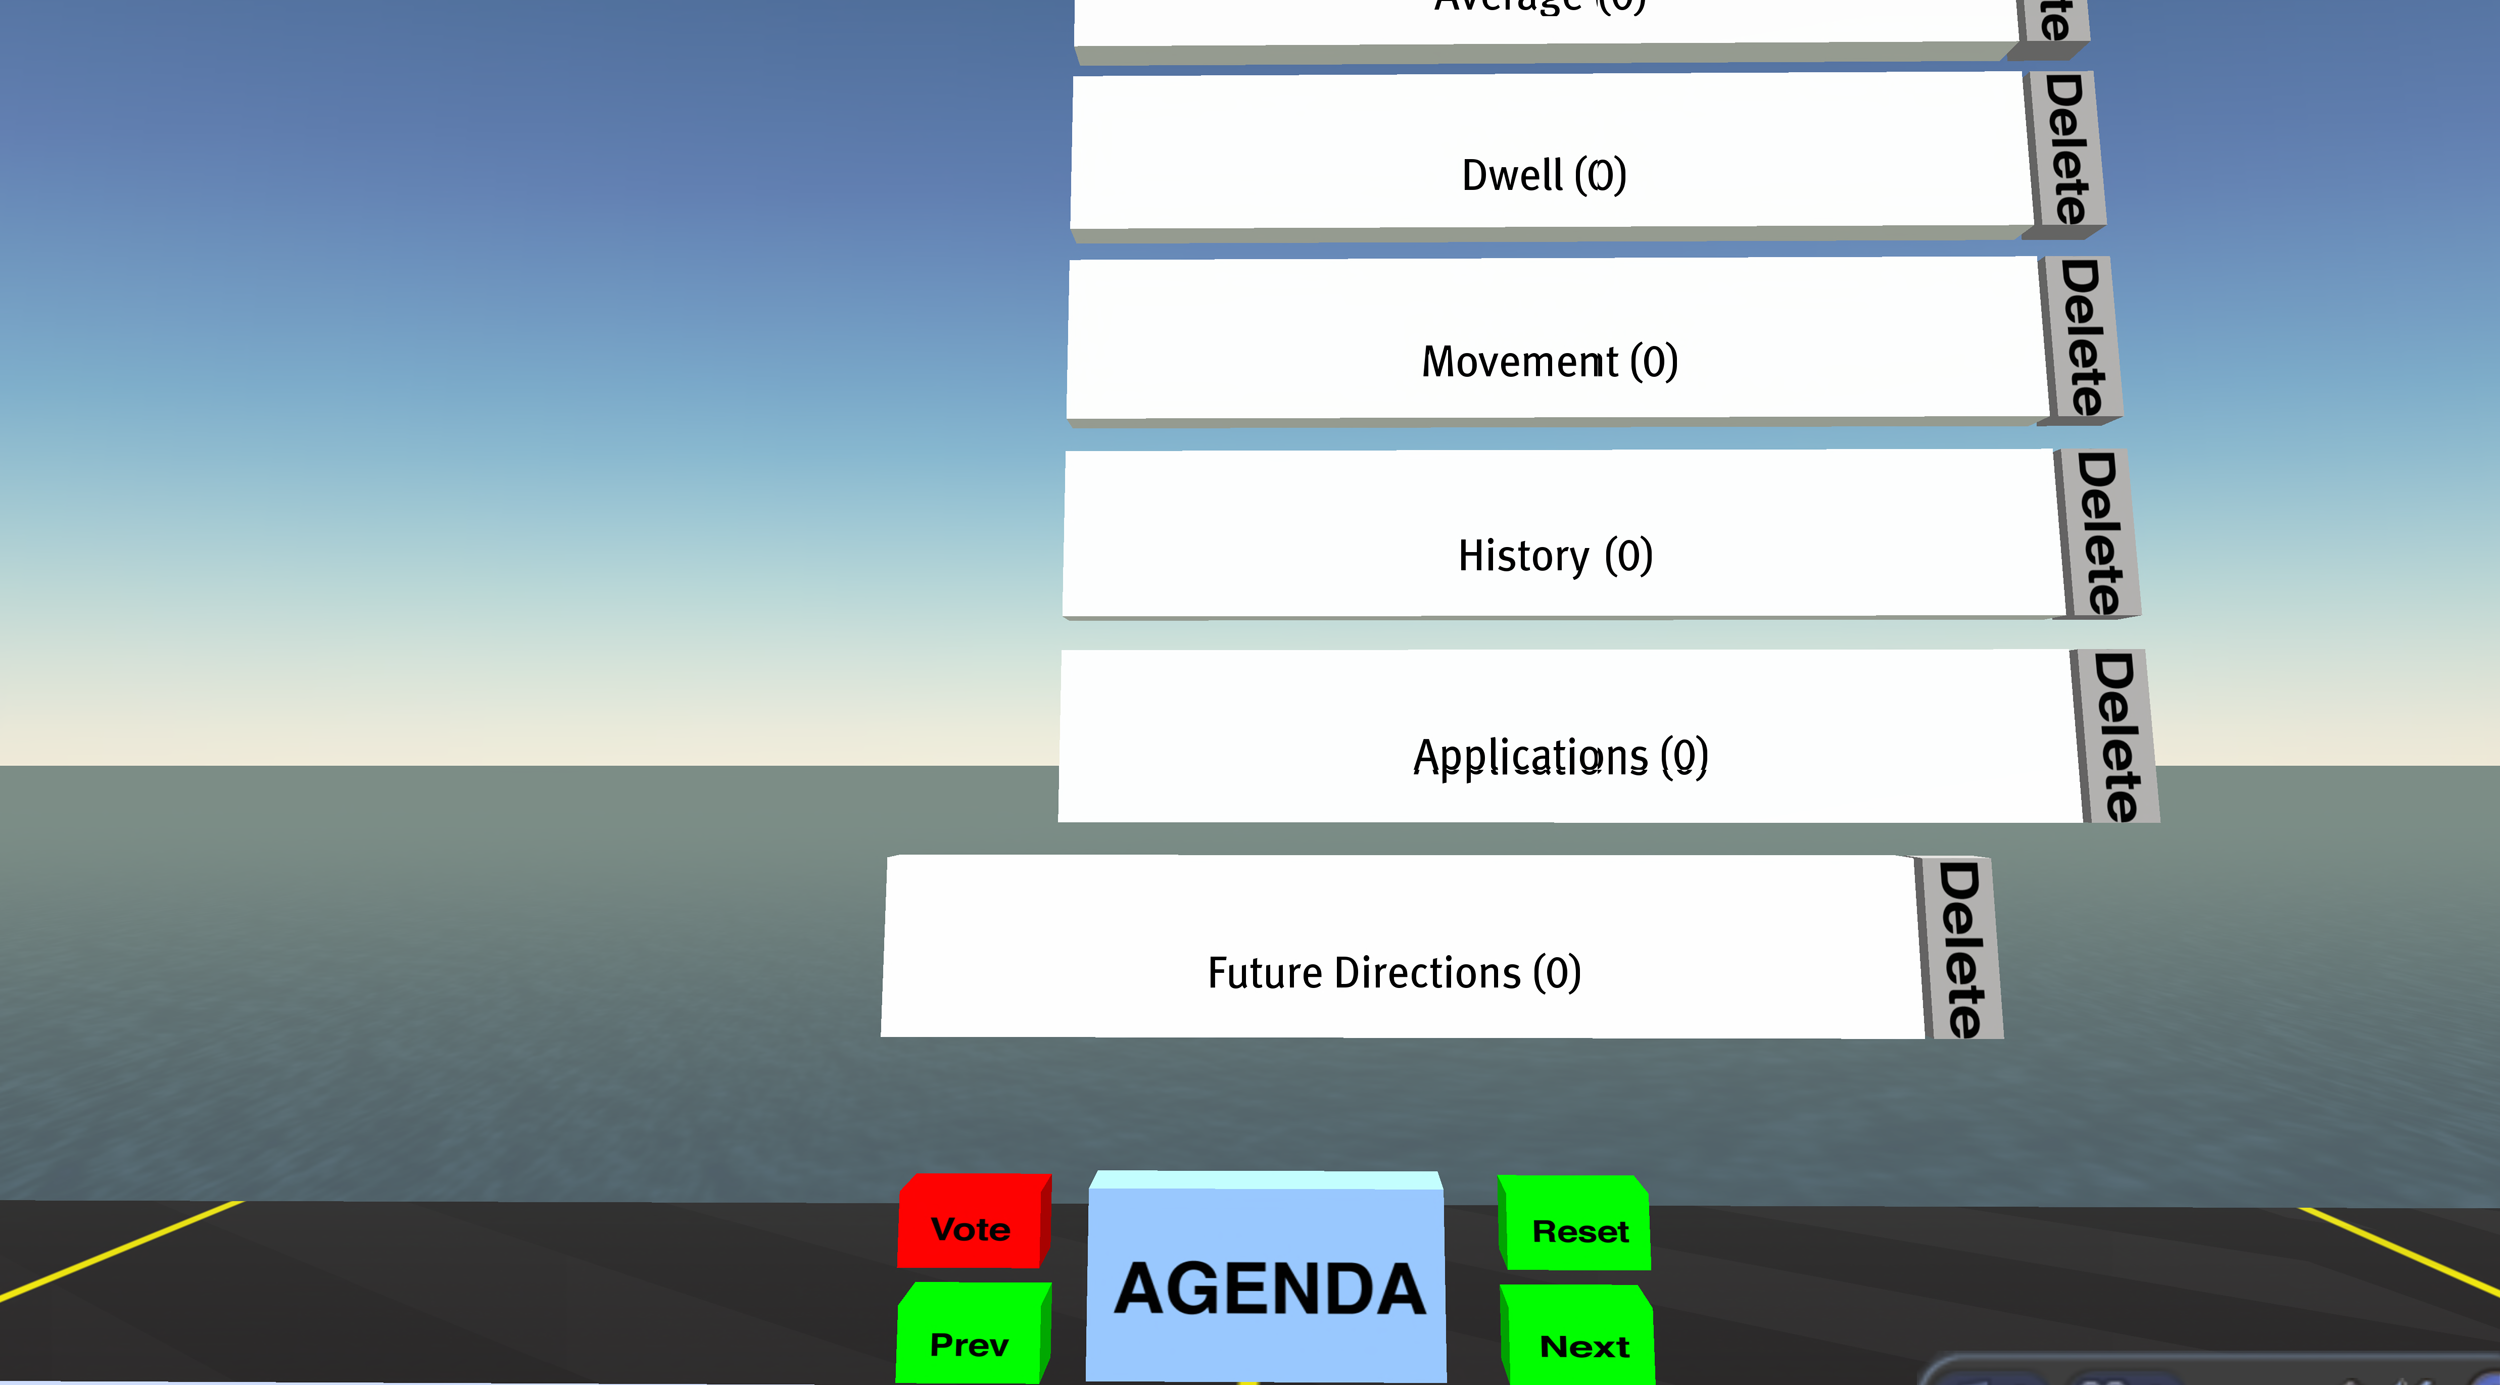
\includegraphics{figures/agenda.png}
	\caption{The agenda system, with buttons for manipulating all items as well as deleting individual items. The text for the agenda is pulled from note cards dropped on the agenda object.}
	\label{fig:information_space_agenda}
\end{figure*}


The dashboard is the heart of the space (Figure \ref{fig:information_space_dashboard}), and contains a range of controls that customize the social experience of being in the space. Each of the social utilities described above can be turned on or off from the dashboard. The texture of the floor itself can also be changed from Agree/Disagree to an other design. The applications are also sometimes connected to the dashboard. The podium that contains the dashboard is also elevated from the floor itself, which reinforces using spatial metaphors the relative roles of the participants---the avatar in that position is understood to have more control over the space.

In a virtual space where avatars can easily act at a distance, the dashboard stands out as an anomaly; only avatars standing within the gray podium (see Figure \ref{fig:information_space_overview}) can push buttons on the podium. This ensures clear attribution to changes in the state of the meeting space. There will never be any question who turned off chat archiving---it had to be the person standing in the podium. From our experiences in physical spaces, we are used to people needing to be proximate to, for instance, light switches to change the lighting in a room. Although this breaks many of the expectations of Second Life users, I believe that enforcing avatar presence near the buttons is an important social cue that helps the legibility of roles and abilities in the space. 

\begin{figure*}[tp]
	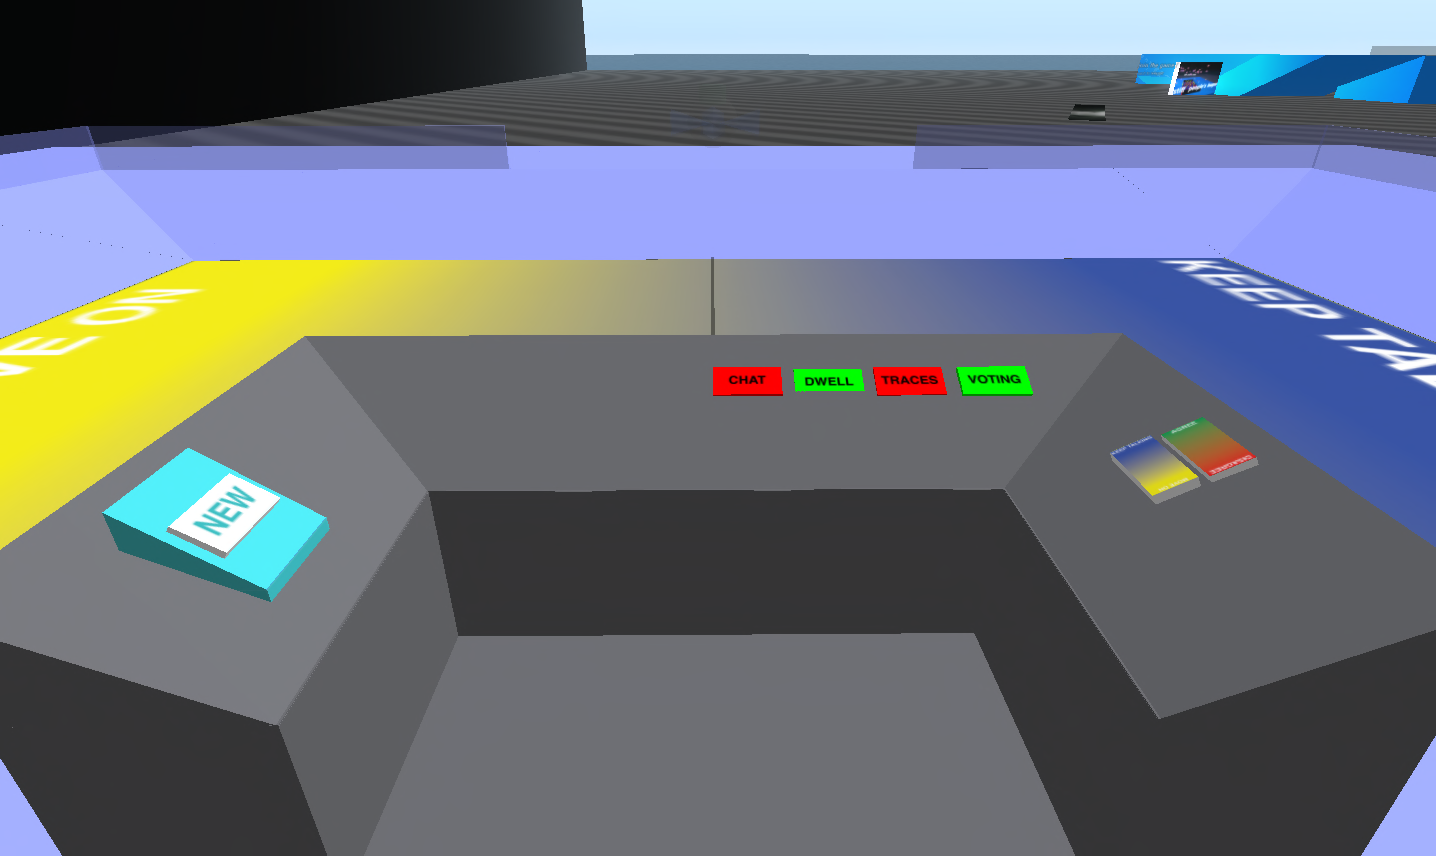
\includegraphics{figures/dashboard.png}
	\caption{The dashboard. Left: A button for making new todo objects. Right: Buttons for configuring the space..}
	\label{fig:information_space_dashboard}
\end{figure*}


\subsection{Deployments}
We have conducted evaluations of this approach. We worked with two existing discussion groups in Second Life to arrange meetings inside an early prototype design. The first group had 7 participants and the second group had 12 participants. Each group was given a list of controversial topics and asked to vote on which one they were most interested in discussing. After choosing a specific topic, they were given an editorial on that topic and then asked to move their avatar to represent whether they agreed or disagreed with the author's argument and to hold a discussion about their opinions on the topic. After the discussion, feedback about the meeting space was collected informally through both individual conversations with participants and group comments.

\begin{marginfigure}
	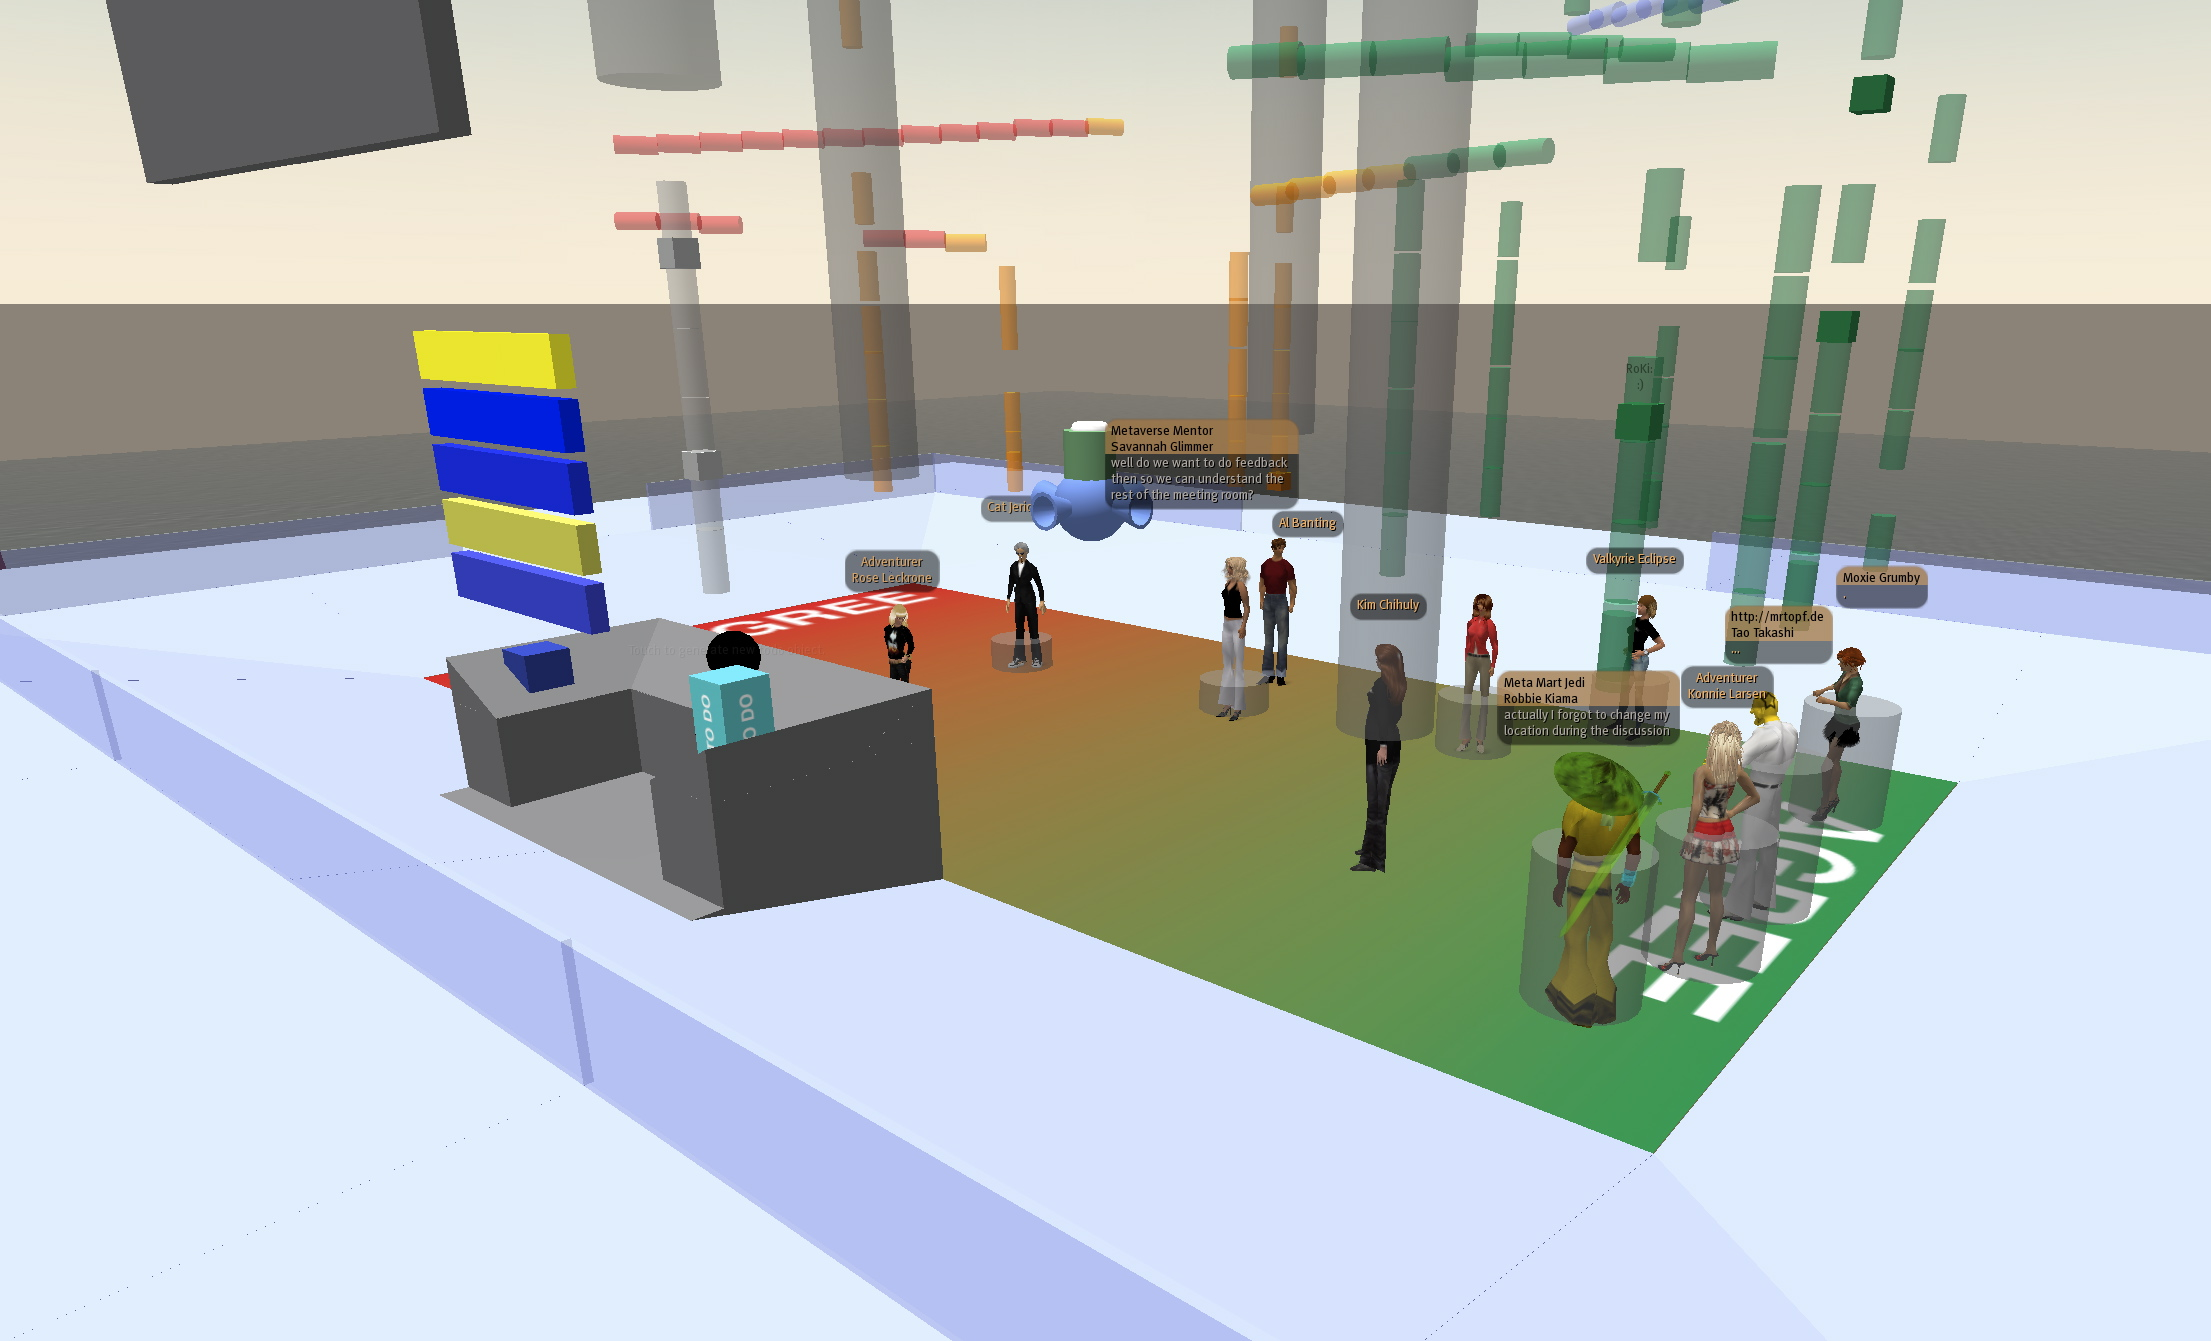
\includegraphics{figures/meeting_space_trial_1.jpg}
	\caption{Screenshot of one of the test deployments. These deployments were done with an earlier version of the system.}
	\label{fig:meeting_space_trial_1}
\end{marginfigure}

Participants were, on the whole, very excited about the potential of the design space. Many of them focused on the social implications of this arrangement, thinking out loud about how they would respond to, e.g., their boss moving to ``agree''. They also appreciated the way the space aggregates history, because they were often pulled away from Second Life briefly and lost track of what was going on.

In these tests, though, participants rarely moved their avatars around the space to take advantage of the many visualization features. This was primarily due to the modality of the Second Life interface. When we were ran these studies, Second Life did not support voice chat (it has since been added), and avatar movement is controlled by the keyboard. Switching between movement mode and typing mode is a little bit confusing. This makes it hard for avatars to both move and talk at the same time.


The other major theme from these experiences was that even relatively sophisticated Second Life users make infrequent use of the elaborate camera controls. As designers, we assumed that all users would be comfortable detaching the camera from their own avatar and inspecting objects in the environment—the conversation archive, in particular. This was not the case with our test groups. Many reported having forgotten about the above-their-heads information because they didn't normally change their camera view. They also reported that their avatar movement was often used to change their camera view, and so making that movement socially significant was sometimes problematic. Instead of visualizing their feelings about the topic, sometimes the space ended up visualizing their attempts to get a better view of the space without using the advanced camera controls.

\begin{marginfigure}
	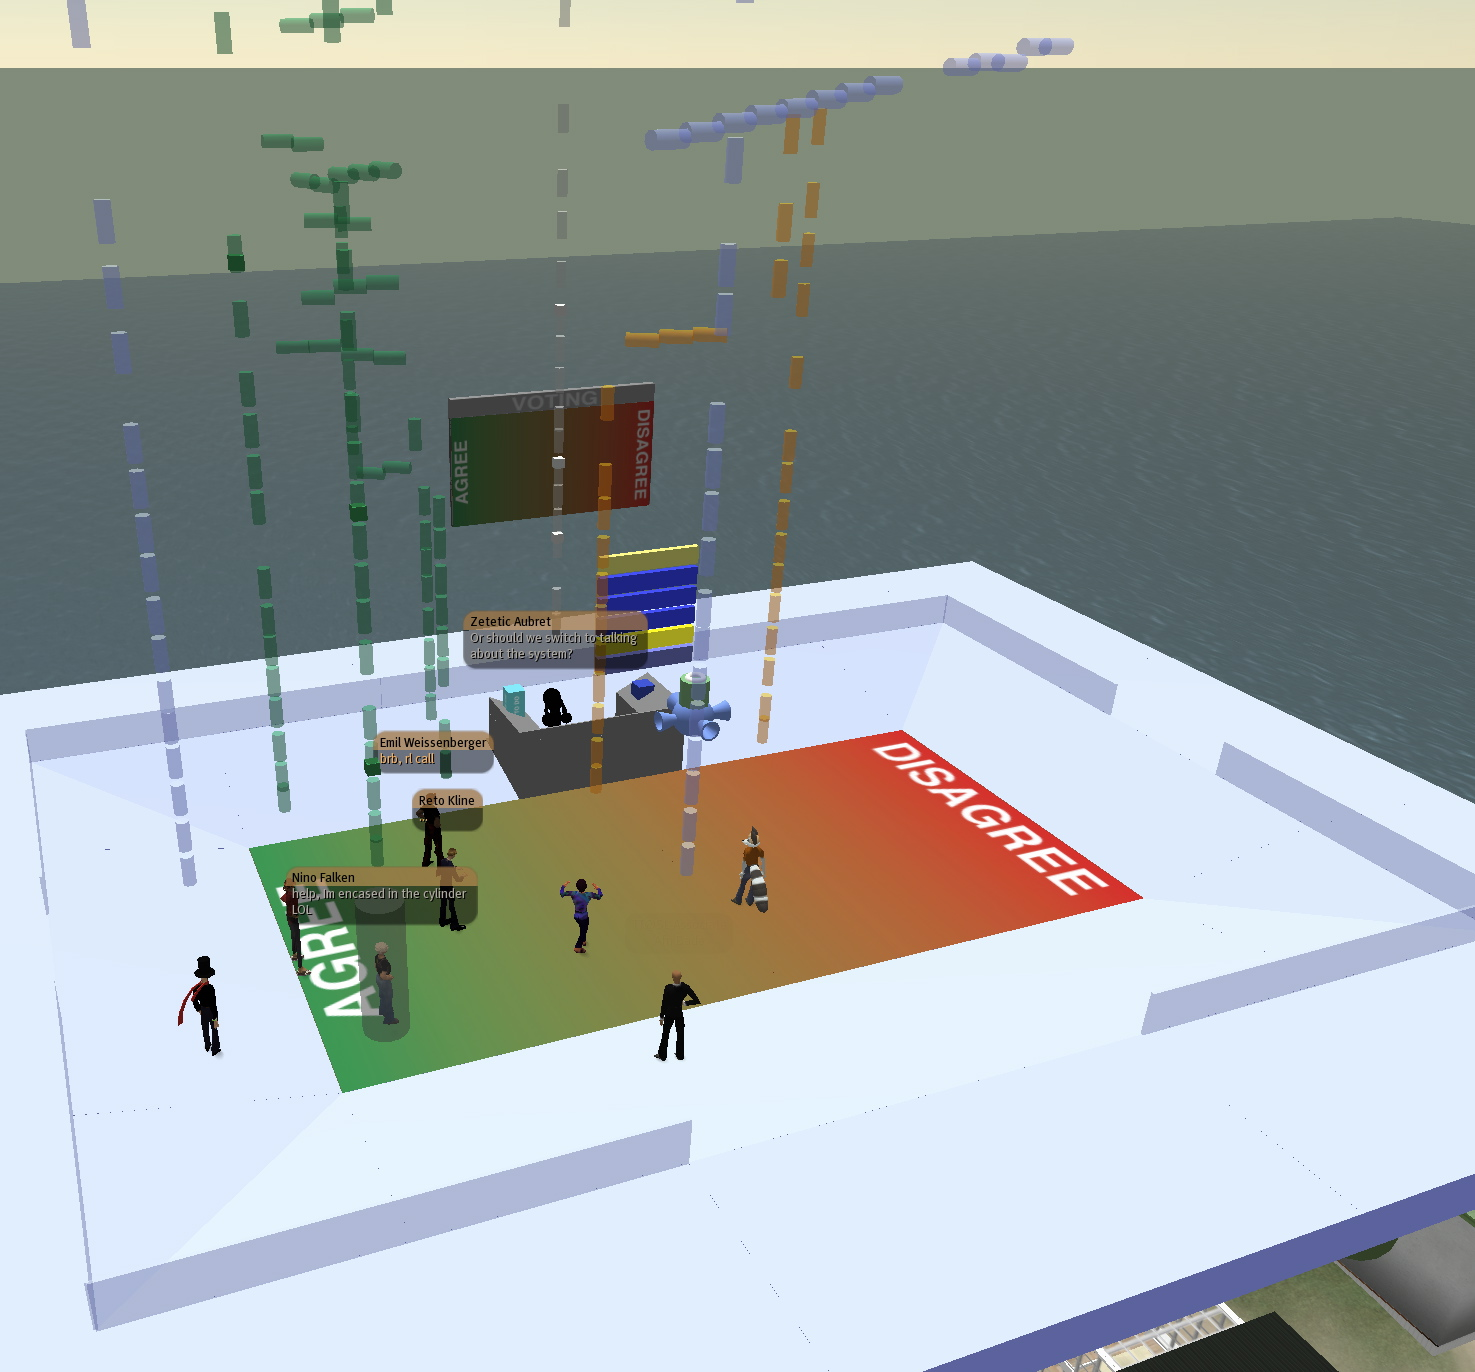
\includegraphics{figures/meeting_space_trial_2.jpg}
	\caption{Screenshot of one of the test deployments. These deployments were done with an earlier version of the system.}
	\label{fig:meeting_space_trial_2}
\end{marginfigure}



As with all domains, applications that challenge users' ideas about what's possible can be hard to understand. In the case of Second Life, this is compounded by user interface issues. This leaves us with a number of possible explanations for users' excitement about the ideas behind Information Spaces but general lack of engagement with specific features. I think the most probable is that because this project reflects both a shift in how to interact with spaces in Second Life as well as forces users to use the interface in ways they might not be familiar, it takes a longer term study than we were able to conduct. Perhaps with a user group that was even more familiar with Second Life and could spend more time acclimating to the environment we could better address aspects of the design in more detail.

\subsection{Analysis}

I propose that there are quite a few different ways in which this design influences the behavior of avatars. As in any meeting situation, the space itself is only part of the picture, and so while all these influences have not necessarily been observed experimentally, it is worth thinking through what the range of possible impacts could be.

One theme common to many of the features of Information Spaces is an emphasis on encouraging more equal participation by showing relative participation levels of participants. Over-talkative meeting participants are reminded of their activity, and people participating less can find space to get their say. This can work on a group level, too. It may be clear by the current average vote in the room that the consensus is squarely on one side, but a vocal minority is out-talking a quiet majority. By color-coding chat messages based on where in the spectrum they come from, the for/against balance can be equalized. Compared to the approach employed by \citet{DiMicco:2007ie}, using shared displays to show relative participation, our approach has a number of benefits. First, mediated participation is far easier to instrument to generate the sorts of graphs in \emph{Second Messenger}. Second, virtual worlds make it easy to render the data in-place, rather than leaving it to users to locate themselves in a displaced representation and map it back onto people. We cannot make a strong argument that this would change the findings from DiMicco, but it is conceptually appealing.

There is an inherent bias in this approach towards meetings in which participants are trying to find better ways to non-verbally express their attitudes. The whole space is focused on making these signals more legible and visible. This is an approach shared by most side stage designs. If the main stage is focused on one speaker at a time, a side stage that supports multiple simultaneous performances can be particularly useful. This does not preclude main stage performances, of course. For participants who are comfortable breaking in on the main stage, it can be a more efficient way to make a point or represent your feelings on an issue. Yet many participants are not always empowered to perform on the main stage, or don't want to wait to take a main stage turn when they can perform immediately on the side stage.

The challenge with this approach is that we are assuming that there is an interest or support for this sort of non-verbal communication. In contexts where the sorts of performances the side stage is designed for are not valued contributions (e.g. in situations where there is a stark power differential within the group), it may be that making these signals more visible is in fact a reason for a participant to be even less open about their feelings. This highlights a limitation in \emph{Second Life}---any system that relies on an avatar's location makes it difficult to anonymize their participation. If side stage performances could be anonymized, they could be a powerful way to balance otherwise imbalanced power relationships. \sidenote{Of course, adoption in tools like this is always a challenge and often requires the buy-in of high status members of an organization. Tools that aim to disempower or level status among a group can be viewed as threatening. This can lead to tools not being introduced at all, or their introduction being systematically undermined. \citep{Orlikowski:1992tza}}

Anonymized participation is a common feature in GDSS systems that is difficult to replicate in a user-friendly way in \emph{Second Life}.\sidenote{This of course presumes that an avatar's identity is what matters. If the mapping between avatar and keyboardist is not made clear, anonymity is manageable. But fluid systems where you can flexibly claim anonymity sometimes but not others (like \emph{Quora}) are difficult to create.}

If there is not group interest in equal participation, it may be that this kind of space would reinforce hierarchies instead of subverting them. While in a face-to-face meeting, substantial effort might be spent trying to figure out what an important decision maker feels about an issue, in this environment they may just move right to that position and everyone else could follow them there, obviating any real discussion of the issues. It may be that if this is really how meetings work, then quickly acknowledging that everyone wants to follow the boss might not be a bad outcome. This effect is limited by the informality of the space. No one is required to indicate a position at any time; instead changes in position (from undecided to decided, for instance) can be done strategically. The system is not designed to be coercive, simply to create a new stage for performances if people want to use it.

By making visible someone's constant attitude about something, meeting participants might be discouraged from moving because dwelling somewhere for a while becomes seen as a status symbol. I suspect that in this situation, the dwell indicator is only making visible pre-existing attitudes about changing ones opinion. In a meeting environment where opinion changes are valued, the bias could just as well be the opposite; staying somewhere too long looks like inactivity and disconnection because the group expectation is that participants will be actively representing and changing their opinion. Participants' use of avatar movement in place of camera control exacerbates this issue; a user that wants to look around will have to give up their dwell indicator, which might cause users who become attached to their dwell indicators to simply not move at all, limiting the impact of the other visualization systems spread around the space. 




\section{Presentation Spaces}

% TODO find the citation for the paper where nicole + jon talk about the problems with presentations in virtual spaces.

For many people, virtual worlds like \emph{Second Life} offered a chance to be part of a broader intellectual life that might not be available to them offline. Although it has faded somewhat, there was a period where lectures and presentations in \emph{Second Life} were reasonably common and provided a platform for people to find interesting social and intellectual contexts without leaving their house. In many ways, this was always the strongest argument for virtual worlds. While they ultimately had a difficult time competing with enterprise collaboration software, \emph{Second Life} in particular had a vibrant community around these sorts of events. Like meeting rooms, the spaces in which these events took place were overwhelmingly literal in their design. \sidenote{The only real concession to the virtuality of the environment was that each ``sim'' in \emph{Second Life} had a population limit, so the best event spaces were located on the corner where four sims met, to maximize the population. You can see across sim boundaries, but not talk.} The speaker typically gave a presentation either through streaming video or (later) used the in-world voice system. Slides were sometimes used, either in a video stream or embedded in the world and managed using in-world tools.

\begin{figure*}[t]
	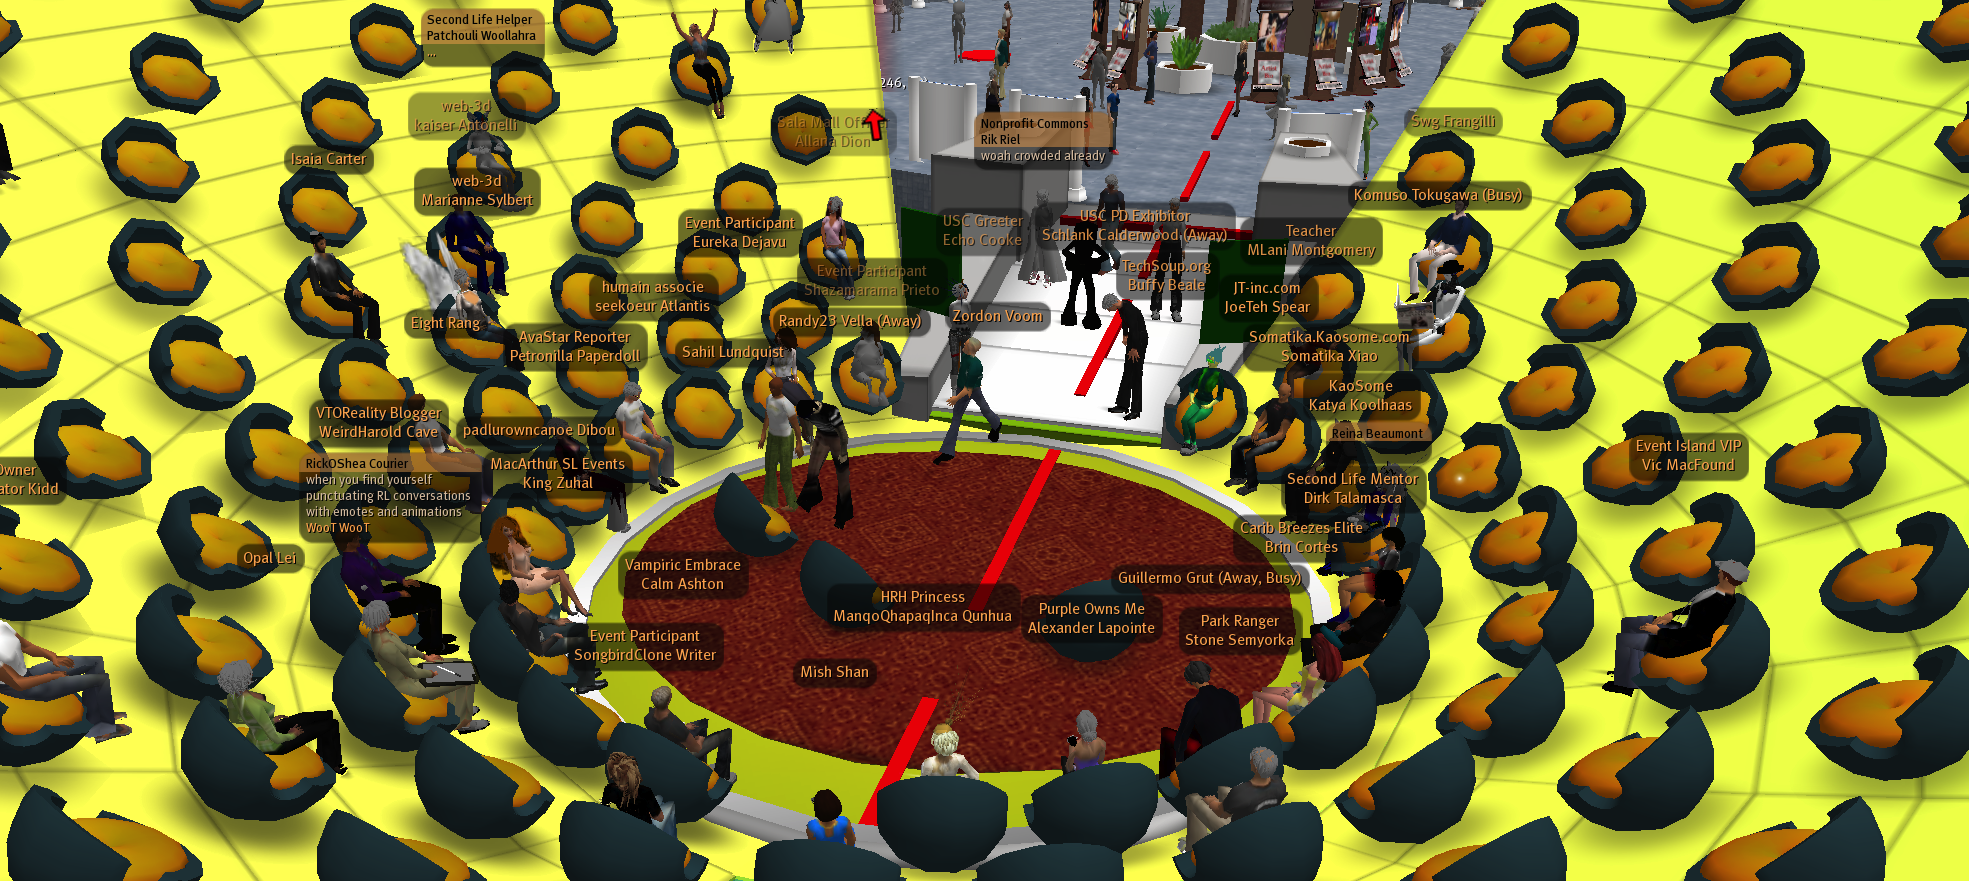
\includegraphics{figures/presentation_1.png}
	\caption{A large amphitheater presentation space at the border of four adjacent sims, with a crowd milling around outside.}
	\label{fig:amphitheater_presentation}
\end{figure*}

\begin{marginfigure}
	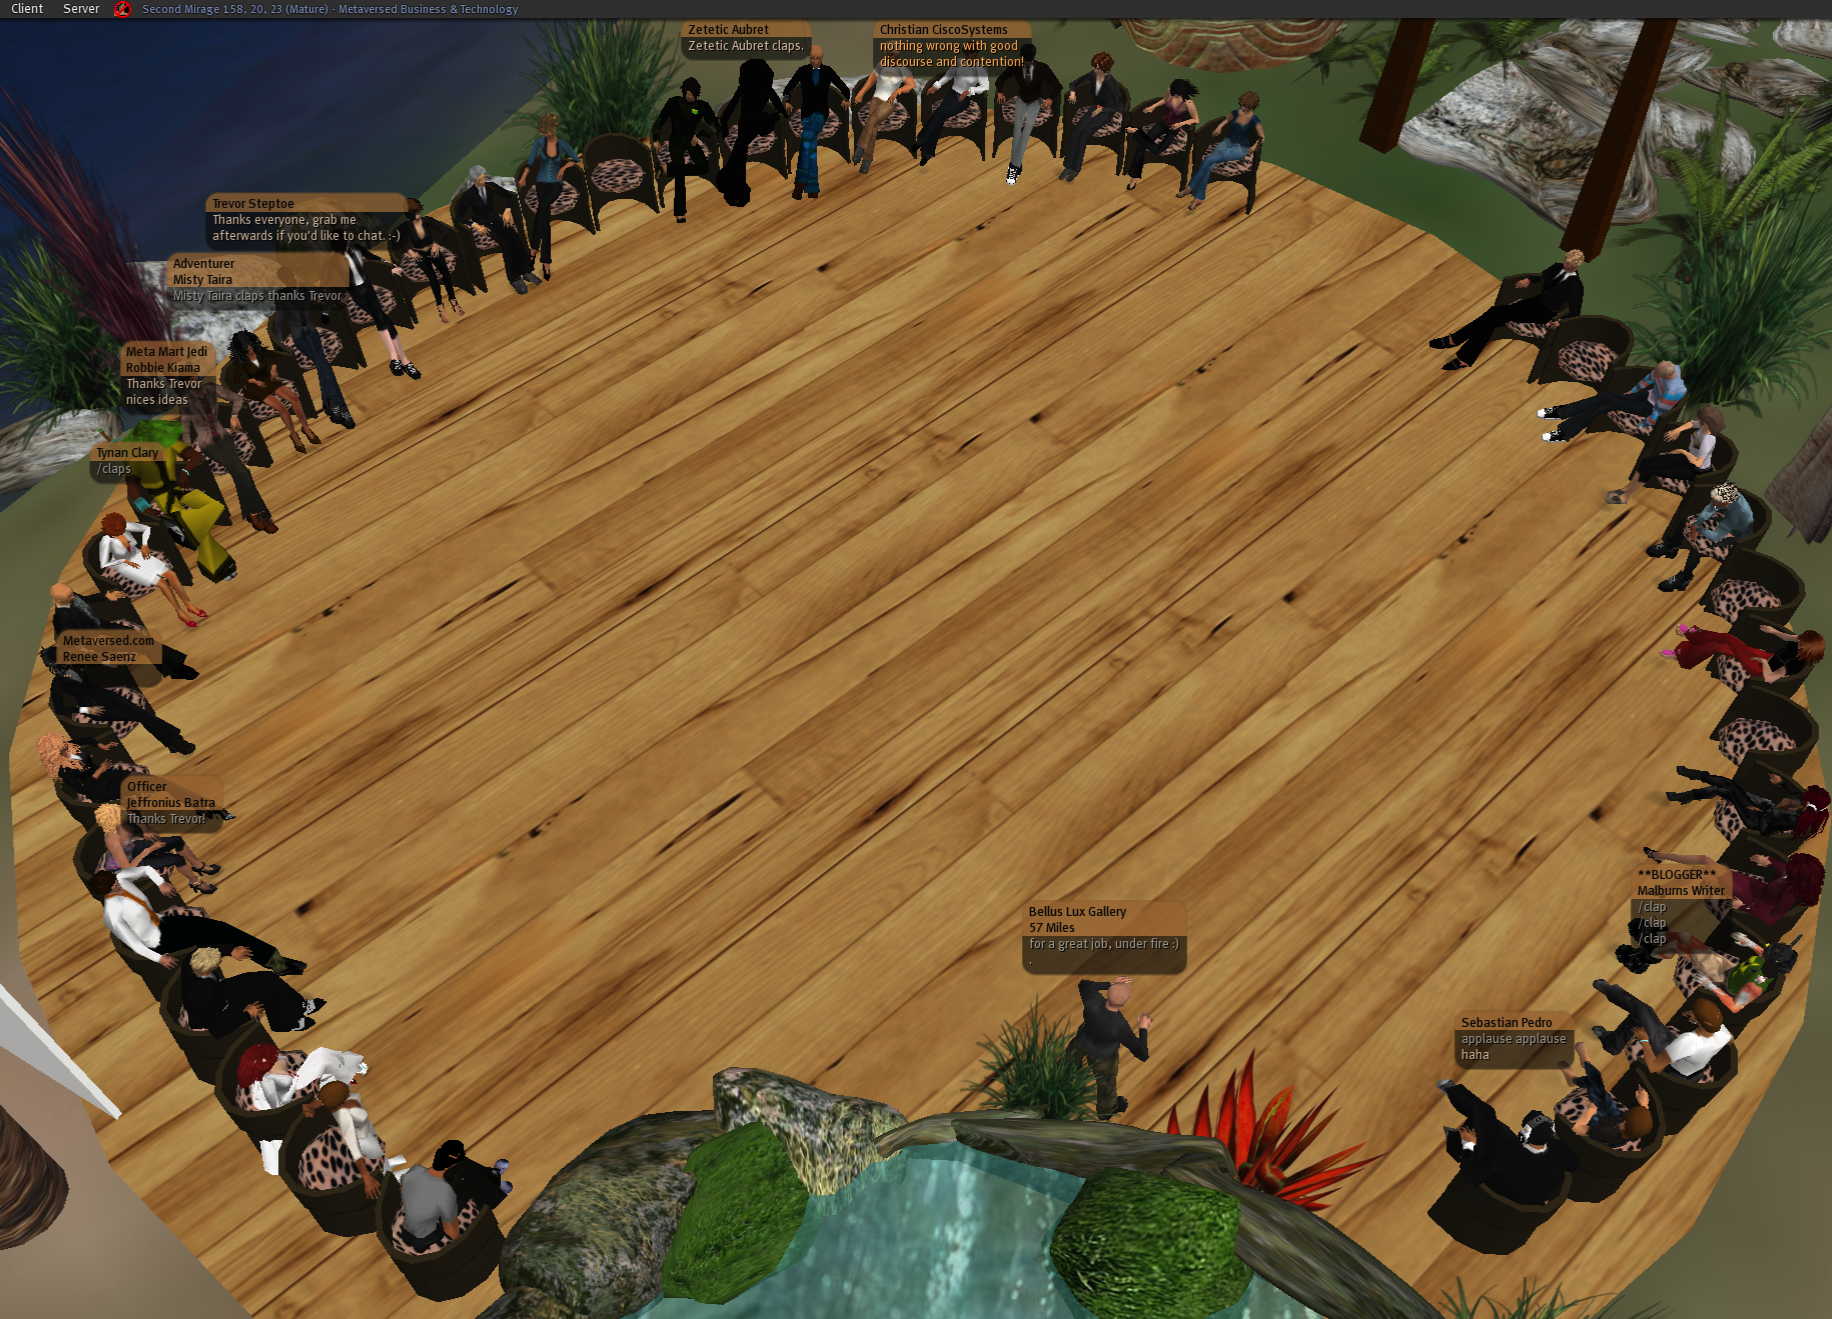
\includegraphics{figures/presentation_2.png}
	\caption{A presentation and discussion space in \emph{Second Life}}
	\label{fig:circle_presentation}
\end{marginfigure}

In this section, I describe \emph{Presentation Spaces}---a system to support these sorts of presentation activities in a virtual world. I take as my starting place the set of challenges laid out by \citet{Yankelovich:2008vk} (with some adjustments):

\begin{description}
\item[Static Presenters]{Managing your avatar in a way that's convincing and demonstrates engagement while also handling the usual challenges of presenting is difficult.}
\item[Dynamic Audiences]{In face to face presentations, our movement is influenced by social norms about having to walk through other people, create noise, etc. In virtual worlds, these tend not to be meaningful limits so people move around much more in ways that is not socially significant but can be quite distracting.}
\item[Communication Confusion]{How can audience members talk to each other? How does that scale up to lots of people? How can the audience communicate to the speaker in a meaningful/useful way?}
\item[Usability]{Virtual worlds make it easy to see people, but building applications in them can be very difficult; managing HUDs/UIs/cameras is typically quite difficult.}
\end{description}

Many of these problems are shared by non-virtual mediated presentations as well. Tools like \emph{WebEx} suffer from many of these issues, too. Although it might be nice to have better audience/presenter interactions, a virtual world context forces these issues. Watching an un-moving avatar representing someone giving a presentation as an audience member is far more disconcerting than watching a slide deck in \emph{WebEx} because there is no ostentatiously awkward representation of that person that they're not attending to. The same is true of the audience. In a traditional conferencing context the audience is essentially invisible, so their absence or activity doesn't get in the way of anyone else's experience. Representing that audience graphically raises the stakes and means we need to either develop ways to incentivize certain sorts of behaviors and discourage others, or think about alternative representations of their activities. 

\emph{Presentation Spaces} seeks to use spatiality to address these issues in an internally consistent way. Instead of assuming a static space, we use the slides of the presentation itself as the primary organizing feature of the space. In an otherwise flat and featureless space, the slides are spread out linearly. The slides form a space that is defined by the slides, and people's positions relative to the slides can become socially meaningful. As in the \emph{Information Spaces} project, there are a series of independent tools that help manage issues like communication confusion, audience movement, and audience/presenter communication. 

Using the stages terminology, the configuration here is quite similar to \emph{Information Spaces}. The main stage includes all the components of the space that are primarily the domain of the presenter: audio content, the slides themselves, and the visual field at the front of the space. The side stage includes all the tools that support non-verbal communication on the part of the audience. Although the semantics of an avatar's position in the space is still a core component of side stage performances, the way those positions are interpreted is quite different from how position and movement were interpreted in \emph{Information Spaces}. The sections that follow will show how the structures in \emph{Presentation Spaces} create a different framework. But the projects share an interest in creating predominantly non-verbal side stages that can enhance the main stage by creating feedback loops in contexts where verbal feedback would be unwieldy. 

This system was built on the \emph{Wonderland} platform \citep{Kaplan:2011en} originally developed at Sun Labs. Although there are significant technical differences between \emph{Wonderland} and \emph{Second Life}, they are broadly similar: they present people with avatars, they support spatialized voice communication, and objects in the world can respond to user input in different ways. The two primary features of \emph{Wonderland} that differentiate in from \emph{Second Life} are its federated, open source server model (compared to \emph{Second Life}'s monolithic, closed source server model) and its broader programmatic access for system developers to more of the internal behaviors of the world (which \emph{Second Life} eschews for security reasons). 


\subsection{Design}

\emph{Presentation Spaces} has four major components: slide spreader, a moving platform, chat zones, and thought bubbles. A new presentation space is created by dropping a PDF into a \emph{Wonderland} world. Slides can be spread in a variety of different ways, and the size and spacing of the slides is controllable. The slides form the backbone of the space, giving it its dominant visual feature. By making all the slides in the presentation immediately visible to all audience members, it becomes instantly clear how long the presentation is going to be and gives an avatar at a certain point in the presentation a sense of context about recent and future slides in a natural way. This sort of use of space is not feasible in \emph{Second Life}, where land is sold by the square meter and this sort of use of space would be extraordinarily indulgent. \sidenote{This is one of the many ways that design decisions about a world can have a major impact on architectural and social practices; builders in \emph{Second Life} frequently build tall instead of wide to manage real estate prices, which exacerbates people's issues navigating and moving in complicated three dimensional spaces with weak camera controls.}

The implicit model with this sort of layout is that the presenter and audience will move from slide to slide over the course of the presentation. Instead of the audience staying stationary and slides changing in front of them, it is the slides that stay stationary and the audience which moves. Think of it like a gallery tour, instead of a slideshow. One of the challenges with organizing a presentation space in this way is the increased navigational burden on audience members. If every slide change required the entire audience to move itself from slide to slide, it would turn changing the slide into an elaborate procedure. You would, however, always know who was present and paying attention because inattentive viewers would rapidly be left behind as the group moves on. But in an experience that is already demanding quite a bit of extra attention from both audience member and presenter, this would likely be overwhelming. 

To help automate the movement process, there is a sliding platform that can move audience members from slide to slide. The platform is controlled by the presenter, so functionally it works just like changing slides. \sidenote[][-1.5in]{We could, of course, move the slides and keep the audience stationary. This is analogous to the camera/document distinction in \emph{Pad++} \citep{Bederson:1998vo}. In this case, the disconcerting effect of moving graphically enormous and solid slides is a strong reason to move the audience instead. Furthermore, moving the slides would make it harder to move among the slides when not on the platform---the slides could move out from under you in a moment.} Audience members on the platform will move naturally from slide to slide, maintaining their view of the current slide, with a glimpse of the next and previous slides. The presenter maintains her perspective too, using an automatic custom camera angle that maintains a view of the audience and of the current, next, and previous slides. Audience members can freely move on and off the platform to more closely inspect past or future slides, or simply to signal that they've stepped away from their computers for a moment as in the border area in \emph{Information Spaces}. 

\begin{figure*}[t]
	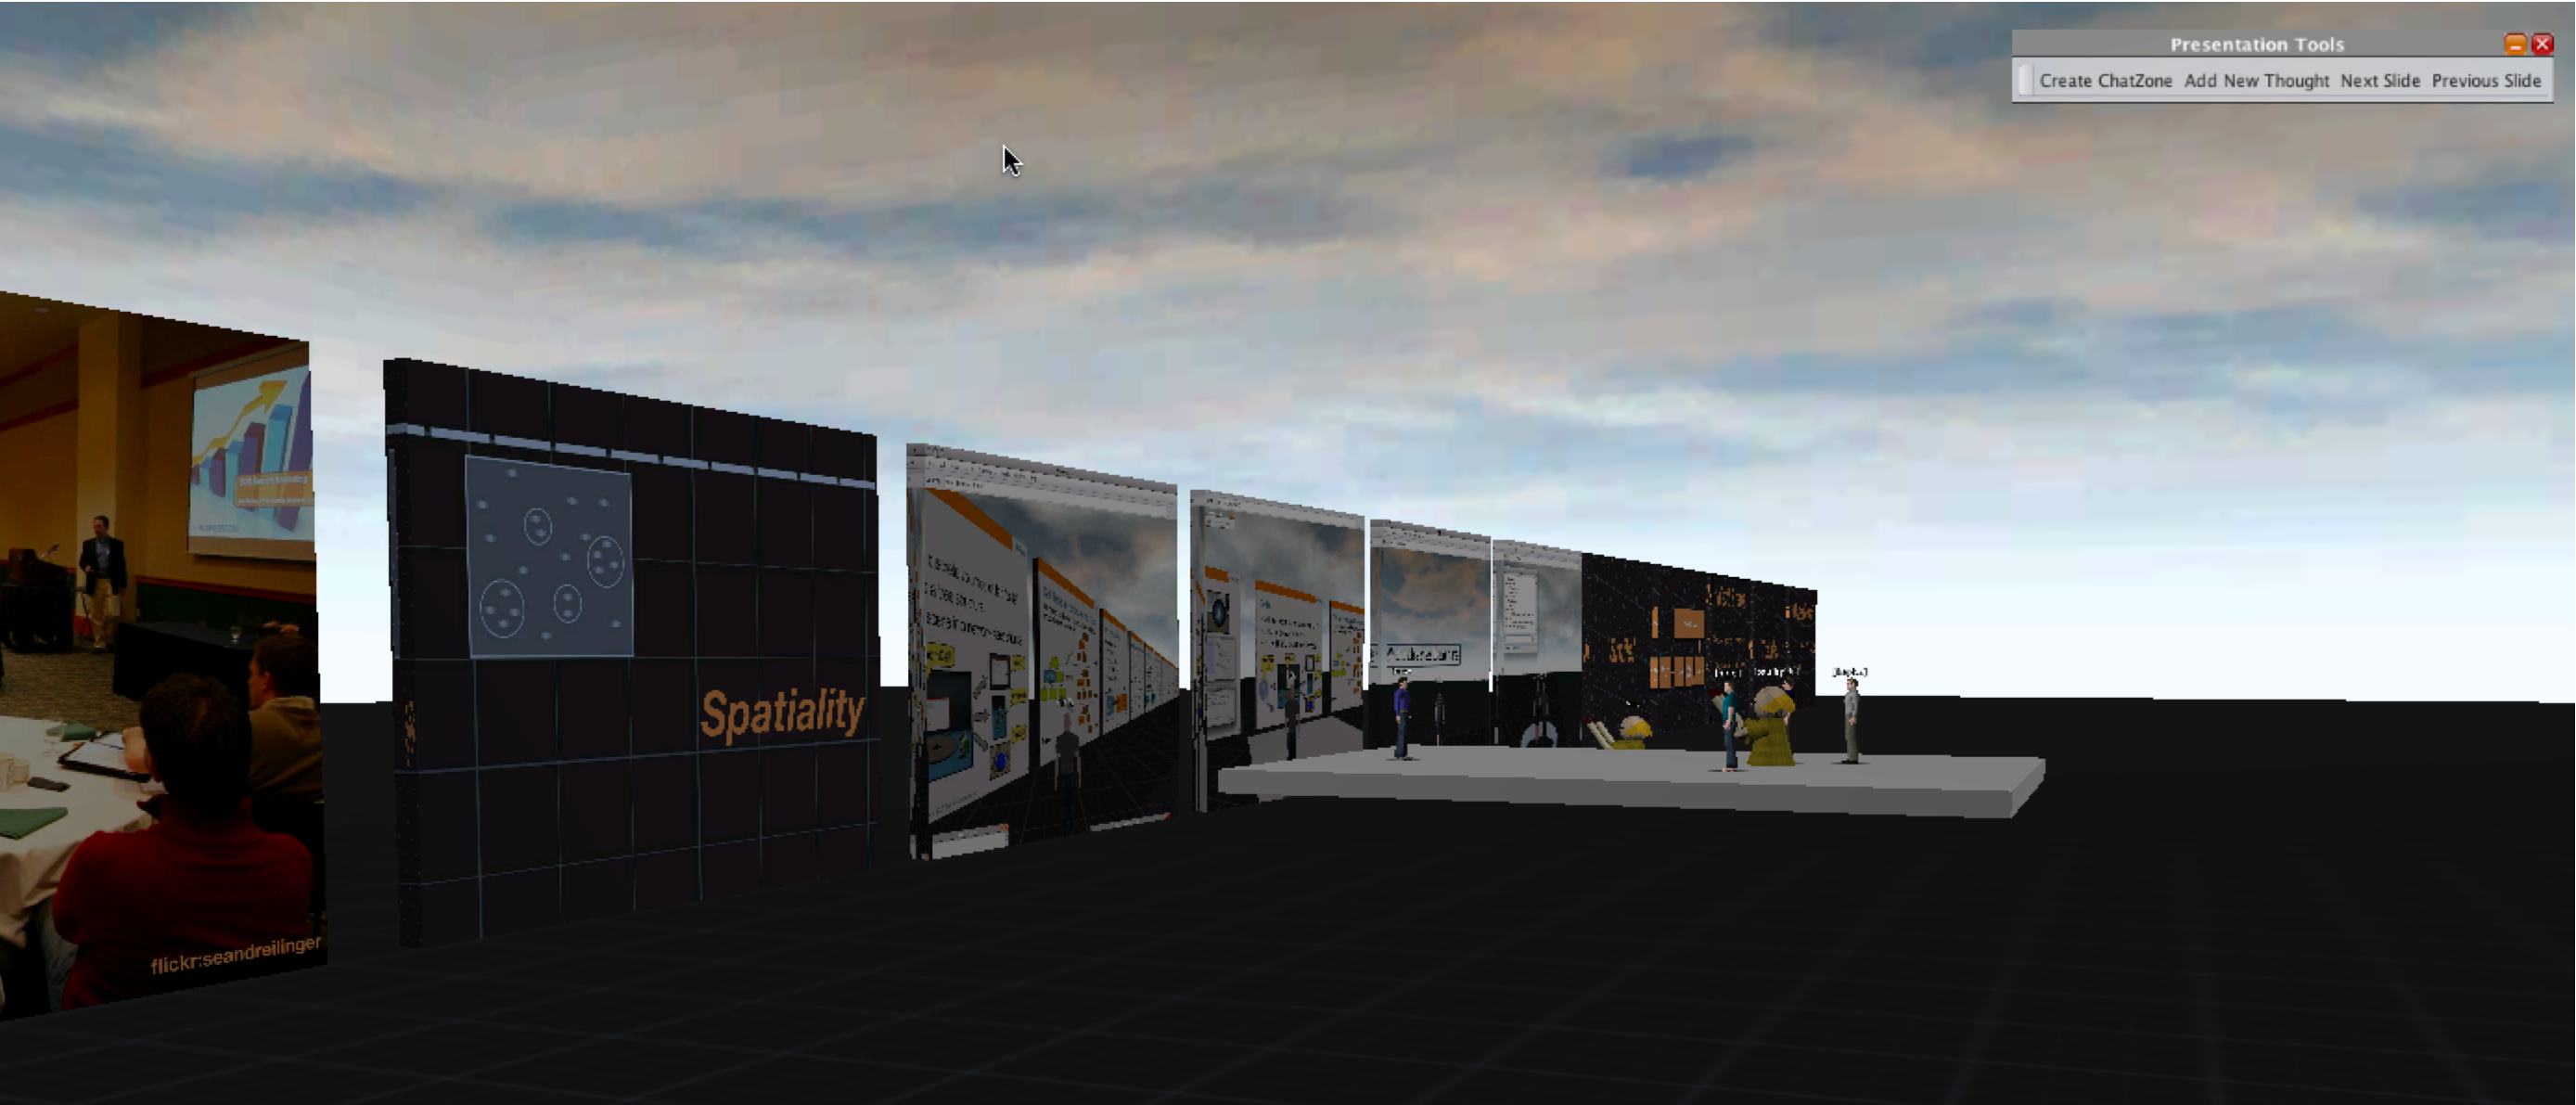
\includegraphics{figures/presentation_screenshot.png}
	\caption{Slides spread out in a space with the platform positioned near the end of the slideshow. Current audience members are standing on the platform watching the presentation. Presentation tools are available in the HUD in the upper right hand corner.}
	\label{fig:presentation_overview}
\end{figure*}

\begin{marginfigure}[1.0in]
	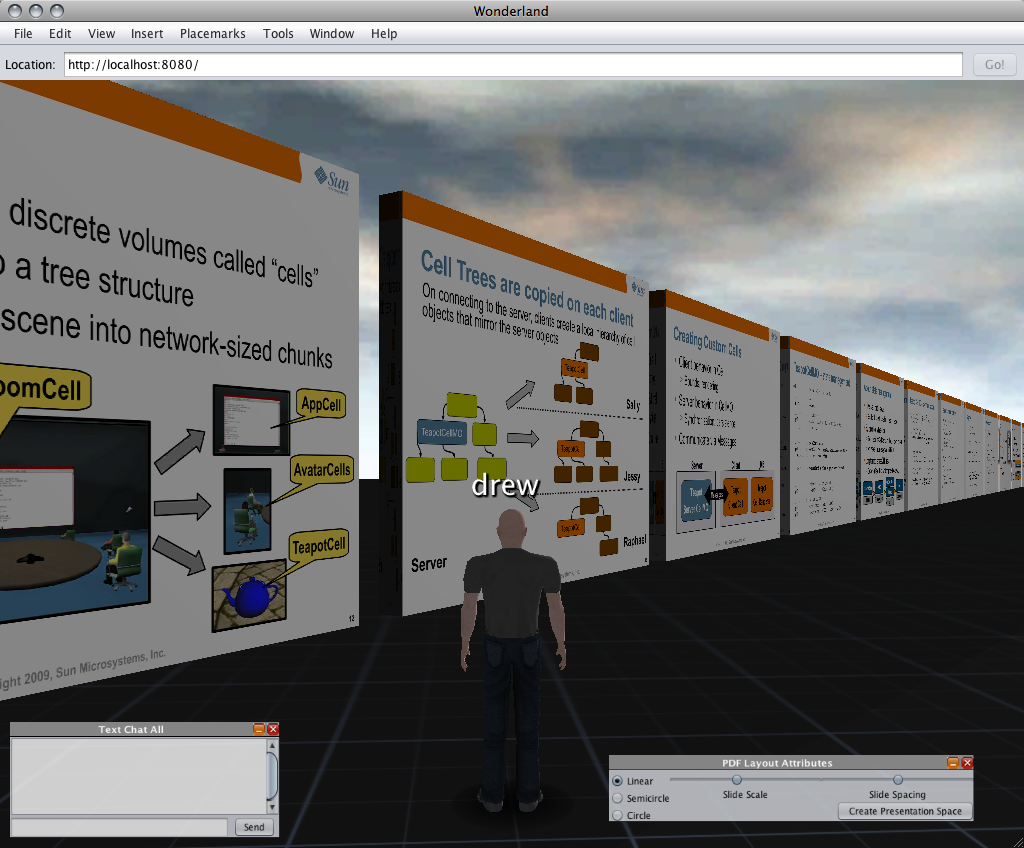
\includegraphics{figures/pdf-spreader.png}
	\caption{A view of the space after dropping a PDF into a \emph{Wonderland} world. HUD controls in the bottom right corner control various settings.}
	\label{fig:pdf_spreader}
\end{marginfigure}

One of the benefits of face-to-face interaction is the ability to carefully moderate your own speaking volume to easily address groups of different sizes. Being able to whisper to a friend sitting next to you at a talk is part of what motivates us to attend events together and sit together. In virtual spaces, this flexibility is difficult to foster. Chat is often spatialized (e.g. people near you can see your chat message, but people farther away cannot), but it's quite difficult to have any intuition about whether someone will be able to hear you or not just looking at their relative position. In physical spaces this is mitigated by being able to \emph{see} that someone is talking but not be able to hear them. This helps us make judgements about the audience for our own spoken comments. \emph{ChatCircles} handled this quite elegantly by representing speaking activity of others at a distance without making the actual content of the communication available. \citep{Viegas:1999kv}

In \emph{Presentation Spaces}, we take a cue from \emph{ChatCircles}, but because of some limitations of the system we render the that ``chat circles'' in a much more literal fashion: as actual circles that avatars can step into and out of. This mimics an approach first seen in the game world \emph{Puzzle Pirates}, shown in Figure \ref{fig:pp_chat_circles}. Using a button on the \emph{Presentation Spaces} HUD interface (seen in the upper right hand corner of Figure \ref{fig:presentation_overview}), any user can create a chat zone underneath their avatar. A new chat zone starts small, but increases its radius whenever anyone walks into it. All zones are public, and can be arranged hierarchically (e.g. zones within zones) or in a disjoint fashion (e.g. partially overlapping). Stepping into a chat zone adds a new zone-specific chat channel to the main chat system. Stepping out of a zone doesn't remove the tab, but it does remove your ability to listen to new messages sent to that group since you left it.

\begin{marginfigure}
	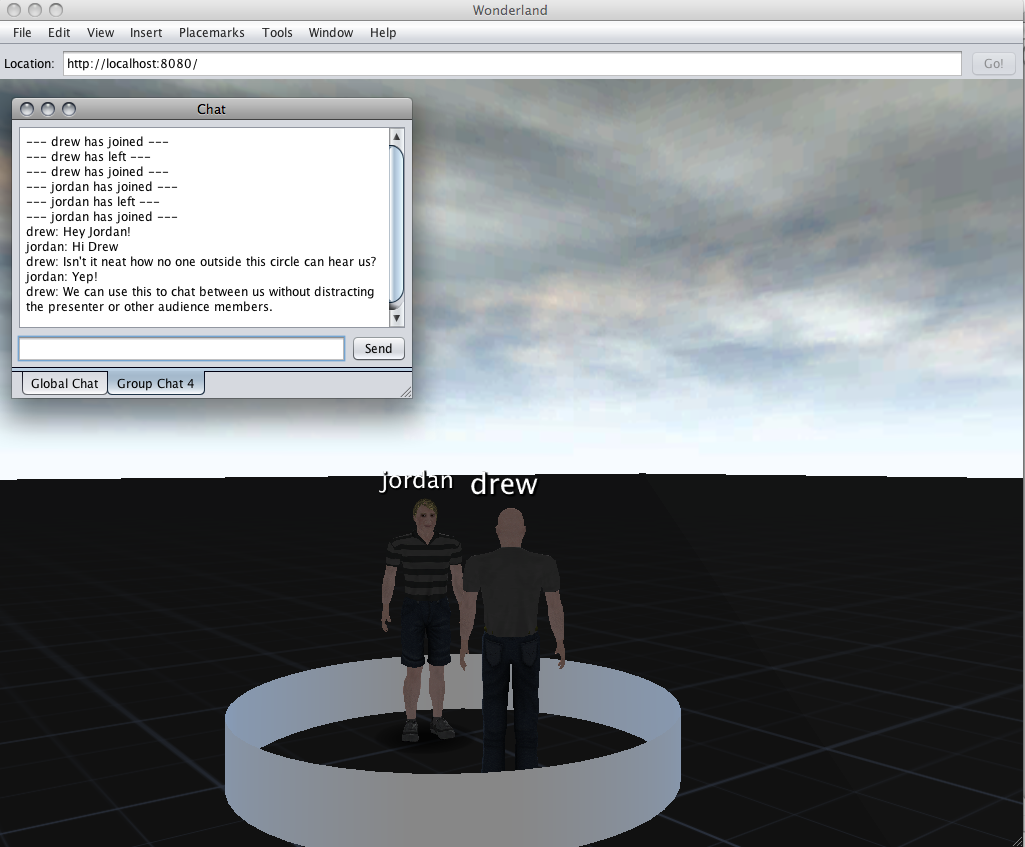
\includegraphics{figures/chat-zones.png}
	\caption{A two-person chat zone. The chat takes place in the chat window in the upper left. Note the distinction between the ``Group Chat'' and ``Global Chat'' tabs. Group chat tabs are automatically added when you enter a new chat zone.}
	\label{fig:chat_zones}
\end{marginfigure}

This sort of interaction is possible without relying on a spatial organization. A simple instant messenger-like experience with invite-only group chat makes it possible to functionally group people and route chat messages in the same way. But this approach suffers from discoverability problems: how can you tell what conversations are going on if they take place invisibly? By linking the distribution of messages to a spatial property like avatars' positions, we make the existence of side conversations visible and discoverable. Using position also organizes the audience in a more sensible way. Instead of avatar position in the audience being arbitrary, an audience using chat zones will be a more legible social space with chat zone boundaries illustrating the broad strokes of relationships in the audience. 


\begin{marginfigure}
	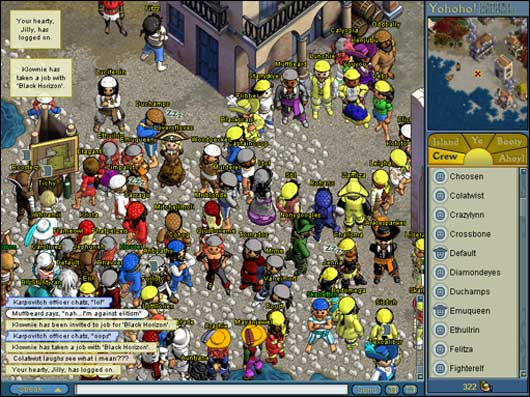
\includegraphics{figures/pp_circles_chat.jpeg}
	\caption{The \emph{Puzzle Pirates} implementation of a related system.}
	\label{fig:pp_chat_circles}
\end{marginfigure}

Chat is a useful mechanism for small groups to interact, but it has two major limitations. It does not persist in a useful way (nor would you want it to, since chat messages are written for a particular audience, not for anybody who comes to the space later), and it is too high frequency for a presenter to keep track of. The thought bubbles system is a way to write messages explicitly to be left behind in a specific space. These messages can be thought of a little more like a tweet in \emph{Twitter} and less like an instant message or chat message. Binding them to a space is another way of using the slides to create contexts for conversation asynchronously. The spread out slides serve as a site for ongoing conversation, both synchronous through chat and asynchronous through thought bubbles. Because thought bubbles are composed in a different way than chat and are a lower-frequency channel, they also become a viable way for different chat zones to interact across zone boundaries as well as for the audience and presenter to interact. Although not fully fleshed out, there's the potential for systems like \emph{backchan.nl} (described in Chapter \ref{ch:backchannl}) to be re-invented in a virtual world context using spatiality and motion to convey the audience's activity in a more dynamic way.


\section{Grounding, Actions, and Attention}

% TODO Update this in light of presentation spaces, too. 

For most of the projects described in this thesis, there is a necessary transposition between the visualization and the world. We are usually limited, in physical spaces, to using projections or screens that require translation between the digital representations of people and any sort of visualization of their behavior. If we take for granted that people identify with the avatars of themselves and other as essentially extensions of their physical body \sidenote{There is good evidence that this is the case. \citep{Yee:2007tl} \citep{Yee:2009vt} \citep{Yee:2007cl} all provide support for this perspective, although there are clearly limits to its effects.} then being able to do in-place visualization seems like a powerful tool. In grounding terms, the appearance and behavior of others is one of the strongest taken-for-granted assumptions in face-to-face conversations; it automatically meets the criteria of being mutually and recursively understood. We may not necessarily parse its content in precisely the same way, but it is clearly a part of someone's appearance and an automatic part of common ground. 

In our deployments of both \emph{Information Spaces} and \emph{Presentation Spaces} we saw little evidence that these representations were a subject of conversation. By analogy, though, it is rare in a group situation to make more than a brief passing comment about someone else's appearance. It may be distinctive and meaningful, but being part of the common ground doesn't mean it's the constant subject of conversation. In fact, the opposite is more likely true; the lack of conversation about people's locations the visualizations based on those locations could also be read as evidence that it didn't \emph{need} to be discussed. It was mutually understood that you had been standing somewhere for a certain amount of time or held a certain opinion. A conversation about these states signals confusion about their meaning or significance.

Although these sorts of visualization strategies are difficult in physical spaces, they are not impossible. The artist Lozano-Hemmer's project Subtitled Public \citep{SubtitledPublic:2005wt} projects phrases on people's bodies, and allows people to transfer these phrases between them by touching other people. This is made possible through an elaborate technical infrastructure of cameras tracking people in the square and a network of powerful projectors. One of the major benefits of virtual world work is that it is possible to conceptualize and experiment with embodied interfaces in a much more rapid and low-cost way. If we accept that this sort of technique is useful, it would be interesting to see how these approaches could be extended in physical spaces. Moving around is clearly more problematic, but providing non-verbal ways to represent your attitudes might be feasible, particularly in already-mediated heterogeneous remote meetings with some local participants and some remote participants.

Given that the primary mode of experiencing virtual worlds is moving around, movement seemed like a natural fit for the primary non-verbal action. Users could be expected to already understand the movement controls. Furthermore, relative avatar movements and locations are meaningful offline social signals.  Although avatars may maintain interpersonal distances per \citep{Yee:2007cl}, that does not mean that movement through the world operates precisely the same way. With our bodies, we can naturally stay in one place while looking around us. This is possible in \emph{Second Life}, but not an interaction that many people found natural. Instead, most residents would simply spin their entire avatar around to look at something behind them and treat their position in the world primarily as a way of setting up their view on the world in a particular way. These two competing desires---to manage their view through their position and to express their attitude about the topic under discussion---were not easily reconciled. By trying to map a pre-existing action onto some new set of meanings, the new meanings faltered and older behaviors tended to take over. This made interpreting movements extremely challenging. Did someone actually change their mind or were they trying to look at one of the active visualizations? This was alleviated somewhat in \emph{Presentation Spaces} with the more elaborate camera controls available in \emph{Wonderland}, but it is also difficult from a usability perspective to be shifting camera angles and expecting people to adapt.

In hindsight, this conflict is essentially irresolvable barring wide-spread education about advanced camera controls. And yet, if we are to give up on position as a primary non-verbal action, there are few other options. The ``touch'' action in \emph{Second Life} is widely used, but suffers from a complete lack of action attribution because avatars can invisibly touch any object in a large radius around themselves. This can be useful for creating opportunities for nearly-anonymous behavior, but is otherwise a sort of thin experience. \emph{Wonderland} lacks any sort of standardized non-verbal action, and instead leaves it to each object to create its own interface. 

These approaches mimic the behavior of traditional applications where each user has a set of inputs and some actions are made visible to other users and some aren't. This is a fine (and clearly effective) model, but doesn't take advantage of the embodiment of a virtual world. If avatars can simply stand in arbitrary locations and manipulate their agree/disagree state, the scene is drained of its social content.

Understanding attention in virtual worlds is tremendously difficult. A conversational participant is not simply attentive or not, attention is something that we use a variety of signals to communicate to others. These signals are almost entirely absent in \emph{Second Life}. Although an avatar's position does suggest the likely view of that user, it is possible for that user's camera to be looking somewhere else entirely. Visualizations of users' movement that expects people to manipulate their cameras independent of their avatar requires this to be the case at least some of the time. This places these two values in contrast: being able to understand the visual fields of others by looking at their avatars and being able to look at visualizations in the environment without moving your avatar. 

This makes it difficult to actively perform attention in the ways we do offline. Performing attention offline involves more than just gaze direction. It involves our entire bodies, our pose, and our face. These are difficult to control in \emph{Second Life}, which makes the performance of attention essentially intractable. In particular, the difference between attention and complete inaction is quite hard to distinguish. Avatars whose users have not touched the keyboard or mouse in quite some time will slouch, but that too is a mixed signal that may just as well represent rapt attention as inattention. Inattention is actually somewhat easier to communicate in the form of manic action. In much the same way it's difficult to imagine that an avatar running around the space is paying any attention. But this is a particularly extreme form of inattention, and more moderate forms of attention and inattention are quite difficult to express.

The ramifications of this lack of expressivity for attention varies somewhat depending on the context. In discussion contexts, conversational participation is a decent (if very low frequency) proxy for attention. We would not expect completely inattentive participants to be able to produce credible contributions to a conversation. But again, a lack of participation is not reliably understood as inattention. These problems are exacerbated substantially in situations where most people are not expected to participate at all, as in a presentation context. Issues with presentations in a virtual world will be addressed in more depth in the next section.

\section{Past and Future Virtuality}

This chapter opened with the breathless claims of a market research firm about the bright future for virtual worlds. This was, at the time, a widely quoted report. There was a large population of skeptics of course, but there were just as many magazines and pundits making similarly bold predictions. When this work was done, I sat somewhere between the skeptics and the optimists. I was interested primarily in virtual worlds as attractive conceptual spaces. Although there was some work that truly pushed the boundaries of how interactions in a virtual space might be different than in offline spaces, the vast majority of the work was focused on mimicking offline designs for social spaces. This made virtual worlds an attractive space to do design-based research. For most of the period when I was working in virtual worlds, I was essentially agnostic about the question of whether or not they would be broadly successful. That was a question on which  someone in my position had no leverage.

Despite my disinterest in prognosticating about virtual worlds, their decline subsequent to this work poses a challenge. Are there ways that this work speaks to non-virtual designs? Are there fundamental conceptual problems with virtual worlds as an experiences that other design approaches that solve similar problems don't suffer from? Are those problems likely to have future technical solutions or are virtual worlds simply a seductive approach that is not broadly applicable?

In this section I aim to provide a series of potential explanations for the failure of this vision to come to pass. Trying to understand a negative result like this in hindsight is an inherently fraught process, but based on my work and the challenges I encountered, I will propose some potential reasons why virtual worlds did not have broader success in the particular contexts I was designing for. I will also try to tease out some lessons from this work that are applicable for non-virtual world work.


The virtual world experience is deeply seductive. It has played a major role in science fiction since \emph{True Names} \citep{Vinge:1987ty}.\sidenote{Other virtual world novels of note include \emph{Neuromancer} \citep{Gibson:1986un}, \emph{Snow Crash} \citep{Stephenson:2000tv}, \emph{Rainbows End} \citep{Vinge:2007wt}, and the \emph{Otherland} series \citep{Williams:1998vf}. A longer discussion of the competing visions of virtuality can be found in \citep{Harry:2008vx}.} Virtual worlds have always represented freedom of various sorts. Freedom from geographic constraints, freedom from scarcity, freedom from your past, and freedom from physical bodily constraints. The virtual would would be the place where you could live in a penthouse apartment, be ravishingly beautiful, and have adventures in exotic places with anyone in the world. 

In fiction, virtual worlds are treated primarily as direct analogs of the offline world. Certain physical laws are relaxed and representations are flexible, but speech, body language, and vision are usually assumed to operate identically. Furthermore, the world itself tends to look and behave like the offline world. \sidenote{The one major exception to this is \emph{Neuromancer} \citep{Gibson:1986un}, in which the world is purely abstract. Gibson's ``cyberspace'' was almost purely a way to interact with data, not with other people. It was geometric and abstract, while almost all other worlds looked ``real'' and have human actors featured prominently.} This vision elided the many practical interface challenges to creating a virtual world that was functionally indistinguishable from the offline world. Instead, there was a tremendous focus on creating something that looked ``real'', not a place that supported ``real'' social interaction. 

This is not to say that interactions in virtual worlds were not or could not be socially meaningful. They can and are. But they don't have the same dynamics as offline interactions and skills in one domain don't transfer easily to the other. People new to a virtual world interface have little intuition about how it operates as a social space, which blunts its efficacy. Just because something \emph{looks} familiar doesn't mean we can reason about it in the same way at all.

The distance between the real world and virtual worlds is clearest at the interface layer. The ways that our bodies interact with the physical world are  elaborate and rich. Virtual world interactions are far more limited. We move using (typically) four keys, or by clicking on where we want our avatar to stand. We move our eyes by spinning our avatar around, or by using elaborate three dimensional camera controls. We animate our avatar with a series of recorded animations identified by names like ``wave'' and ``dance.'' Compared to the expressive capabilities of our bodies, it should not be surprising that having a handful of iconic actions would not make it possible to translate social practices without significant changes. Not just do our bodies appear low fidelity, but our movements are even lower fidelity. \sidenote{It is useful to consider what sport looks like in a virtual context; how do we render the most elaborate ways we use our offline bodies? There exist a variety of video games played professionally in a sport-like way, but none mimic offline sports. They focus on hands instead of full bodies, and have a much more elaborate rule sets than physical sports. They adapt to input techniques available instead of assuming they can meaningfully recreate a physical experience with limited inputs.}

This causes a wide range of insidious problems if we're expecting virtual worlds to work like the physical world we're used to. There are a number of assumptions that start to break down. In the physical world, we assume we know what someone else is seeing based on the angle of their head. In the virtual world, camera view and avatar position are frequently correlated, but not always. In the physical world, we have detailed control over how our bodies are situated and move. This is the foundation for what we think of colloquially as ``body language.'' In the virtual world, avatars tend to be iconic, demonstrating a single named pose at a time that is usually shared by all avatars. Other times, avatars idly animate to make them seem more alive, even if those movements are unrelated to any user input. Communication is radically different, too. As discussed in \emph{Presentation Spaces}, we can build models for who will hear something we say in physical spaces. Online, these models are both difficult to build and hard to come to trust. All of these issues are potentially surmountable and there is interesting research in each of these areas. But given where we're at now, these inconsistencies between the physical and virtual worlds mean we have to treat the virtual world's ``realistic'' rendering as a sort of user interface oddity. Instead of making the interface fall away and be a shortcut to rapidly learning how the world works because of its similarities to the physical world, it is its differences that stand out the most. Virtual worlds are not close enough to the physical world in affordances to make the distinction blurry. Instead, they are much closer to any other mediated communication system, and we should judge their value as a design approach relative to traditional graphical user interfaces. On these terms they seem idiosyncratic and a bit strange.

\begin{marginfigure}
	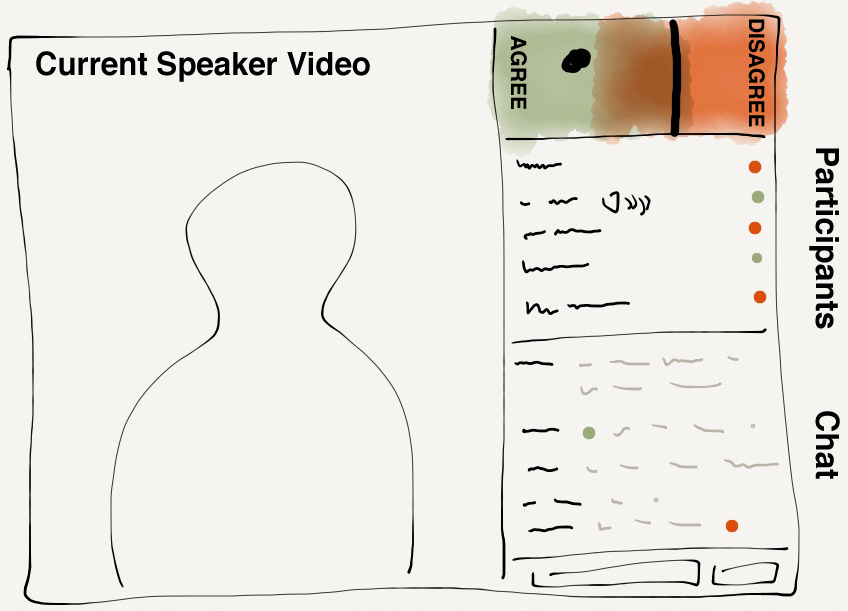
\includegraphics{figures/2d-info-spaces-mockup.png}
	\caption{A rough mockup of what a two dimensional version of \emph{Information Spaces} might look like.}
	\label{fig:infospaces_demake}
\end{marginfigure}

As a thought experiment, it is useful to consider how the systems described in this chapter would (or would not) work as non-virtual world designs. Moving to a 2D GUI approach doesn't necessarily mean throwing away the core design values of spatiality and presence. These principles are essentially ``free'' in a design sense when operating in a virtual context, but as discussed earlier, spatiality doesn't mean three dimensional and presence doesn't mean avatars. Those are simply one technique for creating those experiences. \emph{Information Spaces} could be re-imagined as an addition to a \emph{WebEx}-like experience. A 2D Agree/Disagree continuum could occupy part of the screen, with people's names both creating a sense of presence (who is present) and their showing their current position on an issue. An even less-spatial version might be viable: use the agree/disagree continuum primarily as an input only, and show only the average position. Icons or colors next to people's usernames in the users-present list could provide a person-by-person view. By treating all the inputs of the virtual world as simply actions in an interface, much of the experience can be recreated without any of the elaborate heft of a world.

A similar approach is possible for \emph{Presentation Spaces}. The screen is dominated by the current slide, but viewers can desynchronize themselves from the current slide and explore past and future slides. An indicator shows how many people are currently looking at each slide. Questions or comments can be posted on past/future slides, and can be voted up or down (ala \emph{backchan.nl}). Chat zones would be a little difficult to arrange, but something like an IRC approach with named rooms (similar to \emph{ROAR}, a project I will describe in Chapter \ref{ch:roar}) would be effective. 

\begin{marginfigure}
	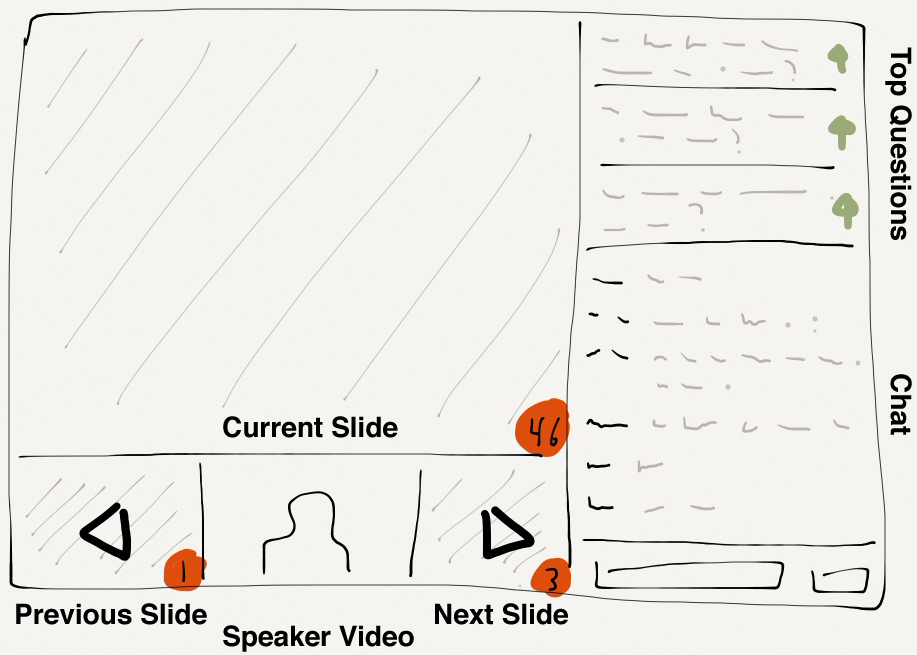
\includegraphics{figures/2d-pres-spaces-mockup.png}
	\caption{A rough mockup of what a two dimensional version of \emph{Presentation Spaces} might look like.}
	\label{fig:presspaces_demake}
\end{marginfigure}


I don't think this sort of adaptation would work for all virtual world experiences. There is something special about a monolithic world like \emph{Second Life} where people socialize, meet new people, play games, and visit notable places all in a continuous, synchronous world. But taken as a venue for traditional mediated experiences like meetings and presentations, there is simply nothing special about it that we couldn't replicate in a traditional interface. Traditional interfaces have the benefit of being much more familiar, not require a powerful computer to handle elaborate 3D environments, and already have rich ecosystems of other tools for these sorts of interactions. This sort of flexibility is even more important now with our plurality of devices; an interface that scales easily to a tablet or phone is easier to integrate into your life than one that requires a powerful computer and large screen. 

This non-virtual-world thought experiment is a way of arguing for the value of this work, despite it taking place originally in a virtual world context. The principles of spatiality (e.g. creating a sense of place and shared audience) and presence (e.g. representing \emph{people}, not just the side effects of their actions) can be useful techniques in a wide range of social experiences. These principles are at the heart of the work in this chapter, and translate well into other domains.


% propose a thought experiment - what would it be like to do the design projets described in this chapter in a 2d environment? Argue that they would be basically attainable and probably more effective because of the explicitness of what's going on. 

% tie this back to why this work is nonetheless worth doing. the non-extraordinariness of virtual worlds means we don't have to place virtual world work in a separate bucket. In fact, the design principles are quite transferable. We can use spatiality and presence in applications with any sort of rendering technique. 


% 
% Having to adapt to a new social system would not be insurmountable, but there needs to be a reason to learn to new social vocabulary. The promise of virtual worlds was that we would learn to manage our avatars and the payoff would be an experience that mimicked offline spaces. But as described before, our thin input language means our experience is quite unlike the real world. Virtual worlds impose serious burdens on our computers, are slow 
% 
% There are two main components to the power of this vision: a freedom from geographic constraints and 
% 
% The idea that we could create technically mediated worlds that would both let us transcend geography but also give us tremendous power over the world itself is at the



